\documentclass[12pt,a4paper,openright,twoside]{book}
\usepackage[utf8]{inputenc}
\usepackage{phd-thesis}
\usepackage{code-lstlistings}
\usepackage{notes}
\usepackage{shortcuts}

\school{ALMA MATER STUDIORUM -- UNIVERSITÀ DI BOLOGNA}
\programme{Dottorato di Ricerca in Data Science and Computation}
\title{On the role of Computational Logics in modern Data Science: representing, learning, reasoning, and explaining knowledge}
\author{Giovanni Ciatto}
\date{\today}
\contestsector{09/H1 -- Sistemi di Elaborazione delle Informazioni}
\scientificsector{ING-INF/05 -- Sistemi di Elaborazione delle Informazioni}
\coordinator{Andrea Cavalli}
\supervisor{Andrea Omicini}
\cycle{XXXIII}
\examyear{2022}

\mainlinespacing{1.241} % line spacing in mainmatter, comment to default (1)

\begin{document}
    
\frontmatter
\frontispiece

\begin{abstract}    
Max 2000 characters, strict.
\end{abstract}

\begin{dedication} % this is optional
Optional. Max a few lines.
\end{dedication}

\begin{acknowledgements} % this is optional
Optional. Max 1 page.
\end{acknowledgements}

%----------------------------------------------------------------------------------------
\tableofcontents   
\listoffigures     % (optional) comment if empty
\lstlistoflistings % (optional) comment if empty
%----------------------------------------------------------------------------------------

\mainmatter

%----------------------------------------------------------------------------------------
\chapter{Introduction}
\label{chap:introduction}
%----------------------------------------------------------------------------------------

In the last decade we have witnessed an explosion in the exploitation of artificial intelligence (AI) both in the academy and in the industry, and in virtually all strategical sectors of human expertise.
%
This is not the first time in history that AI attains unprecedented levels of attention, expectation, and fundings, yet it is the first time that such momentum is driven by a pervasive adoption of data science (DS) and, in particular, machine learning (ML).

Nowadays, the tree terms -- AI, DS, and ML -- are often used mistakenly interchangeably, especially by practitioners.
%
Should we speculate on what the causes of such phenomenon are, we would argue this is likely due to the strong hype characterising modern data-driven solutions---both in theory and in practice.
%
This leads both researchers and practitioners to focus on the development of \emph{ML-oriented} frameworks or technologies which, in turn, create a sampling bias making people think that ML exhausts DS, and DS saturates AI.
%
As we further discuss in the subsequent chapters, this is really far from the truth.
%
There are many interesting aspects of AI which lay outside the realm of DS.
%
Notably, in this thesis we focus on computational logics (CL) -- a prominent aspect of AI populating the portion which is not covered by DS -- and its potential role in complementing DS.

As sub-fields of AI, both DS and CL share the common goal of mimicking human intelligence.
%
Of course, they do so in different ways.
%
They focus on different notions and aspects of intelligence, they pursue intelligence through different ways, and for different purposes.
%
Notably, most differences lay in the way CL and DS treat \emph{knowledge}, and, in particular, in the way knowledge is represented, acquired, manipulated, and transferred.

CL, for instance, focuses on \emph{rational} intelligence, and it aims at endowing machines with human-like, automated \emph{reasoning} capabilities.
%
Following this purpose, it relies on \emph{symbolically} represented knowledge, either acquired via logic induction or via manual handcrafting, manipulated via logic inference (e.g. deduction or abduction), and transferred by simply presenting symbols into shared formats.
%
Dually, DS focuses on \emph{intuitive} intelligence, and it aims at endowing humans with statistical tools for mining significant and predictive information from data, in a principled way.
%
When applied to machines, DS provides them with powerful pattern matching, recognition, or stimulus-response capabilities. 
%
For this reason, it relies on sub-symbolically (e.g. \emph{numerically}) represented knowledge, commonly acquired from data via ML, manipulated via algebraic or differential operations, and transferred in disparate, purpose-specific ways.

Of course, both CL and DS come with shortcomings.
%
On the one side, CL commonly requires
%
\begin{inlinelist}
    \item some symbolic knowledge to be eventually handcrafted by humans, manually; and
    \item the task at hand to have a clear formulation, which can be expressed via crisp symbols.
\end{inlinelist}
%
The former issue, clearly hinders scalability, making CL fall short on the knowledge provisioning side.
%
Vice versa, DS is very well suited on this side, as it naturally leverages on scalable algorithms which have been designed mine information semi-automatically from data, possibly scaling up to very large datasets.
%
The latter issue, in turn, makes CL poorly suited to handle fuzzy tasks which are hard to formalise or encode symbolically---think, for instance, to the task of handwritten digits recognition.
%
On the other side, to be effective, DS commonly requires
%
\begin{inlinelist}
    \item very large amounts of data; and
    \item users to be willing and capable of interpreting the numeric results it outputs.
\end{inlinelist}
%
The former issue actually constrains the exploitation of DS into use cases where data is already available or a provisioning procedure is admissible.
%
Vice versa, CL is data efficient as it can bring valuable results even in presence of very small prior knowledge.
%
The interpretability issue is, in turn, among the most relevant topic nowadays.
%
Given the wide exploitation of DS in some many areas of expertise, clarity and intelligibility of its outcomes are becoming a critical aspects---mostly because of their sub-symbolic nature.
%
Vice versa, CL is inherently symbolic in nature and therefore less subject to such interpretability issues.

Accordingly, this thesis stems from the acknowledgement that CS and DS are complementary -- rather than competing -- aspects of AI, and that \emph{knowledge} plays a pivotal role in both these fields.
%
Along this line, we aim to \emph{elicit} and \emph{enable} the many possible bridges among them, w.r.t. knowledge manipualtion.
%
In doing so, we follow the ultimate purpose of increasing the degree of intelligence and autonomy of modern computational systems.
%
Therefore, our focus is on computational entities and on the ways they can combine and integrate CL and DS to either act more intelligently or more autonomosly---or both. 

On the one side, we \emph{elicit} analogies, dichotomies, and possible synergies among CL and DS by analysing them along four orthogonal dimensions, corresponding to as many knowledge-related activities, namely:
%
\begin{description}
    \item[representation] | i.e. the way knowledge is expressed and made interpretable by either machines or human beings, or both; e.g. via symbols, formul\ae, or tensors of real numbers 

    \item[acquisition] | i.e. the way novel knowledge is learned from prior information, mined from data, or attained from external sources; e.g. via data mining, via induction, or via interaction 
    
    \item[inference] |  i.e. the way decisions, suggestions, recommendations, or predictions can be automatically computed out of prior knowledge; e.g. via automated deduction/abduction, or via classification/regression
    
    \item[explanation] | i.e. the way knowledge can be transferred to another entity---be it computational or human
\end{description}

On the other side, we acknowledge that both CL and DS have a prominent overlap with computer science (CS) and software engineering (SE).
%
Regardless of how they manipulate knowledge, both approaches subtend a mathematical modelling of many computational aspects, which must then be reified into well-engineered software technologies to let practitioners actually exploit them. 
%
Accordingly, we further analyse CL and DS from both a computational and technological perspective.
%
While the computational perspective focuses on \emph{what} data structures, algorithms, and workflows they leverage upon to attain intelligence, the technological perspective focuses on \emph{how} such aspects can be translated in practice, via robust software architectures and effective implementations.
%
Along this line, in particular, we assess the current state of the art for technologies laying at the intersection among DS and CL -- or supporting the construction of bridges among the two fields --, identifying holes and proposing lacks to overcome them.
%
The latter in particular is the contribution by which we \emph{enable} the actual combination of CL and DS in practice.

We carry out the whole discussion under an agent-oriented mindset.
%
Within the scope of this document, we call ``agent'' any autonomous entity having its own \emph{locus of control}---be it a human being or a running process programmed software.
%
We may refer to agents as ``intelligent'' in case the come equipped with human-like knowledge-related capabilities, such as the aforementioned capabilities of representing, learning, inferring, or explaining knowledge---or, possibly, a multitude of them.
%
Under such a mindset, human agents are intelligent by definition, whereas software agents may tend to intelligence by acquiring one or more of these capabilities via either CS or DS---or, hopefully, a combination of them.
%
Accordingly, what we have so far called ``machines'' are indeed ``software agents'', and the overall role of the agent-oriented mindset is about focussing on \emph{who} is charge of manipulating knowledge and \emph{when}, other than \emph{where} should knowledge be located in the meanwhile.

\note{Discuss the goal of the thesis}

\paragraph{Structure of the thesis}

Summarising, the whole thesis discusses in what ways CL and DS can jointly contribute to the management of knowledge within the scope of modern and future intelligent systems, and how technically sound software technologies can be realised along the path.
%
An agent-oriented mindset permeates the whole discussion, by stressing pivotal role of autonomous agents in exploiting both means to reach higher degrees of intelligence.
%
Accordingly, this thesis is organised in three parts, named \emph{What}, \emph{How}, and \emph{Who}, respectively.

In the first part (\emph{What}), we focus on the computational perspective.
%
There, we present the two main branches of AI---namely, the \emph{symbolic} and \emph{sub-symbolic} ones.
%
In particular, we recall classical definitions and survey the current state of the art for both CL and DS.
%
We finally present their strengths and weaknesses, and the many possible bridges among them, w.r.t. knowledge representation, acquisition, manipulation, and transfer.

In the second part (\emph{How}), we focus on the technological perspective.
%
There, we survey the current state of technologies.
%
In particular, we focus on logic-based technologies laying at the intersection with DS, identifying the current lacks w.r.t. current theoretical advances. 
%
We then propose the notion of AI ecosystem, and \twopkt{} as its main reification in software.
%
Finally, we present a number of possible ways to extend the \twopkt{} ecosystem towards DS.

Finally, the third part (\emph{Who}) closes the loop by discussing the role of agents \ldots
\note{TBD}


\part{What}
\label{part:what}

\chapter{Historical Perspective on AI}

AI is a multi-faceted discipline leveraging on contributions coming from several areas of human knowledge, there including Mathematics, Computer Science, Statistics, Psychology, Philosophy, and many others.
%
A famous and comprehensive survey on the many aspects of AI is proposed by Russell and Norving in \cite{russell2016artificial}.
%
In the second half the $20^{th}$ century -- when AI was firstly recognised as discipline by itself -- several approaches towards machine intelligence became subject of intensive research efforts, leading to the vast corpus of literature and to the abundance of techniques available today.

Notably, two main families of approaches has initially emerged in AI, namely, the \emph{symbolic} and \emph{connectionist} ones \cite{Smolensky1987, SUN2001783}.
%
While the former focuses on representing the world through symbols -- in turn representing concepts --, thus emulating how the human \emph{mind} reasons and infers, the latter aims at mimicking human intuition by emulating how the human \emph{brain} works at a very low level.
%
Despite both families have both pros and cons, they have stepped through both glory and misery---in terms of expectations, funding, research interest, and industry adoption \cite{Hendler2008, russell2016artificial}.

For instance, despite the initial hype, artificial neural networks (NN) -- the warhorse of connectionism -- encountered their first \emph{winter} when Rosenblatt's \emph{perceptron} \cite{rosenblatt1957perceptron} was proven unable to learn the XOR function \cite{Minsky1988}.
%
The period following the publication of the well-known Back-Propagation algorithm \cite{Bryson1979} and the proof that multi-layered perceptrons could be used as universal functional approximators \cite{Cybenko1989}, can be considered as the second \emph{spring} of connectionist approaches.
%
However, at the time -- likely, because of computational limits of the hardware and the lack of data -- the success of connectionist approaches can be considered very moderate, especially when compared with the explosion of deep NN and deep learning (DL) \cite{goodfellow2016deep} which was pervasive in both the academy and the industry during the 2010s, and can thus be considered the third spring of AI.

Even if it is currently not as popular as NN, the history of symbolic AI is extremely important as well---mostly because of the prominent influence it has on the many fields converging in AI.
%
Despite their original ambition of reproducing human reasoning \emph{in toto} has been was inevitably rejected by facts, symbolic approaches gave birth to several research lines which are nowadays considered autonomous fields, such as computational logic \cite{lloyd1990computational}, logic programming \cite{apt1990logic}, planning \cite[Chap. 10-11]{russell2016artificial}, multi agent systems \cite{ferber1999multi}, etc. 

A few decades later, many things has changed.
%
ML, DL, Data Mining \cite{hand2006data}, and Bayesian Inference have enormously widened the spectrum of tasks AI can handle, other than the amount of use cases where AI can be applied.
%
Nevertheless, a dualism is still there, alive and healthy, dividing symbolic approaches from what are now called \emph{sub-symbolic}  ones.

Nowadays, sub-symbolic techniques include NN, but they are not limited to the connectionist techniques.
%
The panorama of sub-symbolic techniques has been widened by the development of several data-mining algorithms -- along with their efficient implementations --, such as SVM \cite{Smola2004}, K-Means, Expectation Maximisation \cite{Dempster77maximumlikelihood}, Viterbi \cite{Viterbi06}, etc, which mostly leverage on \emph{numerical} computations while not being backed by a biological metaphor.

Summarising, at the gates of 2020s, AI consists of a number of powerful techniques -- often backed by sound theoretical or empirical backgrounds --, which are widely employed to automate disparate tasks, both in the industry and in the research.
%
Such tasks, and, in particular, the techniques supporting them, can be categorised within two mostly disjoint families---namely the symbolic and sub-symbolic ones.

\subsubsection{Weak vs.\ Strong AI}

A fundamental question in AI concerns the ultimate goal of the discipline itself.
%
Some say AI should (tend to) produce machines which are actually able to think intelligently -- thus adapt to different situations, understand the context their are situated into, learn from the interactions with the environment and with others --, while say it would be sufficient to create machines simply acting \emph{as if} they were thinking intelligently.
%
The former perspective is classically known as \emph{strong} AI, while the latter is known as \emph{weak} AI.
%
Searle's Chinese Room argument \cite{searle1980} clearly explains the difference among the two by means of a practical example, whereas the well known Turing test \cite{Turing1950} provides a practical means to decide whether a machine's AI is actually strong or not.

Even without discussing the many important and subtle philosophical issues arising from such a dualistic view of AI, we note what follows.
%
The original goal of AI was reaching strong AI.
%
This is likely why, initially, so much hype was put in both symbolic and connectionist approaches.
%
But this is also justifying the strong disappointment which led AI towards its first winter.
%
Most researchers soon realised that weak AI was a far more affordable deal, and this is likely why they stopped seeking generality and started focusing on how to improve each single technique, tailoring them to the domains where they could bring more advantage.

A few years later, the global effect is that a plethora of techniques is available to effectively and efficiently tackle as many tasks.
%
But the glue keeping everything together is still human intelligence \cite{Yao2018}.
%
Indeed, symbolic techniques still require human beings to \emph{handcraft} most complex rules or to \emph{manually} build large knowledge bases.
%
Similarly, most ML-powered models still rely on data scientists to lead their training process.
%
Data scientists are still needed, for instance, to clean-up and pre-process data, and to set up predictors hyper-parameters through their experience, or to leverage on their intuition to interpret how a trained predictor is functioning.

Summarising, the success of AI nowadays is also due to its reduced expectations with respect to what can be delegated to machines.
%
As a side effect, poor care is dedicated in studying how AI could be used to \emph{automate} the many processes involving several, interrelated AI-powered tasks.

\subsubsection{Symbolic vs.\ Sub-symbolic AI}

In the recent years, the historical dichotomy between the ``two souls'' of AI has been reconciled, in favour of a comprehensive vision where symbolic and sub-symbolic approaches are seen as \emph{complementary} -- rather than in a competition -- so that they mutually soften their corners \cite{Hoehndorf2017, xailp-woa2019, lpaas-bdcc2}.
%
While symbolic approaches are well suited for relatively small-sized problems where complex and exact tasks has to be performed, possibly relying on structured data -- like for instance planning a sequence of actions, finding a path in a graph taking several constrains into an account, deducing information from a prior knowledge base, or learning mathematical relations from vary small data sets --, sub-symbolic approaches are best suited for those use cases where big (up to huge) amounts of possibly unstructured data  must be processed, where errors or lack of precision is tolerated to some extent, if unavoidable---like for instance classifying images or texts, profiling customers by looking at their shopping history, forecasting the weather for a particular area, etc.
%
Such issues, are not affecting symbolic techniques---especially when symbols are wisely chosen in order to steer humans' intuition.
%
This is because symbols are far closer to what our conscious, rational mind used to handle.
%
For all such reasons, many researchers along the history of AI have argued that a comprehensive approach unifying the two worlds would bring great advantage.

More precisely, complementarity between symbolic and sub-symbolic AI naturally emerges when comparing the two approaches under the following perspectives:
%
\begin{itemize}
    \item sub-symbolic AI is \emph{opaque}, meaning that human beings struggle in understanding the functioning and behaviour of sub-symbolically intelligent systems; instead, symbolic AI is more \emph{transparent}, as it is both human- and machine-interpretable at the same time
    %
    \item sub-symbolic AI can improve itself \emph{automatically} by consuming data, but it is difficult to extend and re-use outside the contexts it was designed for; conversely, symbolic AI is flexible and extensible, but requires humans to \emph{manually} provide symbolic knowledge
    %
    \item sub-symbolic AI is adequate for \emph{fuzzy} problems where some (minimal) degree of error or uncertainty can be tolerated; whereas symbolic AI calls for precise data and queries provided by human beings, yet provides exact, \emph{crisp} results as its outcome.
\end{itemize}

In the remainder of this chapter, we provide a brief overview of the two major disciplines laying within the scope of symbolic or sub-symbolic AI, respectively.
%
These are computational logic -- a prominent branch of symbolic AI leveraging on logics to per form any knowledge-related task, ranging from representation to inference --, and data science -- a prominent branch of sub-symbolic AI leveraging on statistics to manipulate data and mine knowledge out of them.

\section{Computational Logic}
\mypapers[section]{cco-softwarex-2021-2pkt,Korner2020HistoryFuturePrologTPLP,logictech-information11}

\emph{Computational logic} (CL) \cite{lloyd1990computational} is a fundamental research area for \emph{artificial intelligence} (AI), dealing with formal logic as a means for computing \cite{Paulson2018}.
%
Its penetration into \emph{symbolic AI} is nearly pervasive nowadays, and increasingly going deeper within \emph{sub-symbolic AI} \cite{xaisurvey-ia14,lptech4mas-jaamas35}: CL has enabled the development of the former in the past, and it is now pushing the latter towards interpretability and explainability.
%
Be it exploited to manipulate symbols, or to make sub-symbolic solutions human-intelligible, the common expectation behind CL is to endow software systems with \emph{automated} reasoning.

Generally speaking, automated reasoning involves three major aspects:
%
\begin{inlinelist}
    \item logics,
    \item inference rules, and
    \item resolution strategies.
\end{inlinelist}

\emph{Logic} formally defines how knowledge is represented and how novel knowledge can be derived from prior one.
%
Each logic comes with several \emph{inference rules}, dictating how to produce new knowledge under particular circumstances.
%
When coupled with some \emph{resolution strategy}, inference rules become deterministic algorithms that computers can execute to reason autonomously.

Many logics exist in CL -- e.g. propositional, first-order (FOL), temporal, deontic, etc. --, each one targeting a specific way of reasoning.
%
For instance, temporal logic enables reasoning about the chronological ordering of events, deontic logic supports reasoning about permissions/prohibitions and their circumstances, while FOL is general-purpose.
%
Furthermore, different sorts of inference rules exist for different logics.
%
Some are \emph{deductive} -- drawing conclusions out of premises --, some are \emph{inductive} -- looking for general rules out of several premises-conclusion examples --, while other are \emph{abductive}---speculating on which premises caused some conclusions.
%
Finally, when a resolution strategy exists for some rule and logic, it can be reified in software, and used to build intelligent systems capable of automated reasoning.
%
Software of that sort are commonly referred to as a part of the \emph{logic programming} (LP) paradigm~\cite{Nerode1996}.

In LP, programs are typically \emph{theories} (a.k.a.\ \emph{knowledge bases}, KB), i.e.\ collections of sentences in logical form, expressing \emph{facts} and \emph{rules} about some domain, typically in the form of \emph{clauses}, i.e. expressions connecting a number of interrelated \emph{predicates} via logic connectives (e.g. operators such as $\wedge$, $\vee$, $\rightarrow$, $\leftrightarrow$, $\lnot$, etc.).
 %, i.e.:
% \[ \mathit{Head} \impliedBy \mathit{Body_1},\ ...,\ \mathit{Body_n} \]%,
% where both $\mathit{Head}$ and $\mathit{Body_i}$ are \emph{atomic} formul\ae{}, and the whole sentence is read declaratively as logical implication (right-to-left).
% %
% If $n = 0$, the clause is called \emph{fact}, \emph{rule} otherwise.
% %
% An atomic formula is an expression in the form $P(t_1,...,t_m)$ where $P$ is a $m$-ary predicate ($m \geq 0$), and $t_j$ are \emph{terms}.
% %
% Terms are the most general sort of data structure in LP languages.
% %
% They can be \emph{constant} (either \emph{numbers} or \emph{atoms}/strings), \emph{variables}, or recursive elements named \emph{structures}.
% %
% Structures are used to represent clauses, lists, sets, or other sorts of expressions.
%
There, predicates represent statements describing or relating one or more entities about the domain at hand.

Depending on the particular logic of choice, predicates -- and therefore clauses -- may, carry \emph{variables}, i.e. placeholders for unknown entities, and possibly quantifiers for those variables ($\exists$ or $\forall$).
%
Some logics may also endow clauses with further information, such as for instance \emph{probabilities} -- describing the degree of likelihood for a clause to hold true --, or \emph{modalities}---describing the context in which a clause may hold (e.g. \emph{when}).
%
In any case, logic information is represented in such a way that both human and computational agents can interpret and manipulate it, in principle.

One powerful trait of logics is that they enable the representation of complex, intricate, or infinite domains \emph{intensively} (i.e. implicitly) rather than explicitly---e.g. via multiple recursive clauses.
%
So, if a domain involves an infinite amount of entites, these do not necessarily require an infinite amount of memory to be represented.
%
For instance, the set of natural integers can be represented in logic using just two FOL clauses---of which, one is recursive.

Software agents devoted to automated reasoning via LP are commonly referred to as logic \emph{solvers}.
%
They rely on pre-existing KB to derive inferences via some inference procedure and resolution strategy.
%
They may do so either \emph{reactively}, -- i.e. in response to some external stimulus, e.g. some user's \emph{query} --, or \emph{pro-actively}---i.e. spontaneously, in order to reach some goal, e.g. computing the optimal path before moving. 
%
Prolog-based solvers \cite{ColmerauerR93,colmerauer1986-theoreticalProlog}, for instance, exploit a \emph{deductive} procedure rooted into the SLDNF resolution principle \cite{Kowalski1974, Clark77}, and a depth-first strategy.
%
They commonly do so in response to users' queries, provided via a textual interface.
%
Yet, a number of Prolog solvers exists supporting the same inference procedure via different strategies (e.g. tabled-resolution\missingref) or as well as entirely different principles (e.g. Constraint Logic Programming). 
%
Of course, other options exist targetting other logics as well, like, e.g., abductive \cite{FungIff97}, inductive \cite{Muggleton94}, probabilistic \cite{RaedtK15} inference.
%
Each of them represents a particular reification of a logic solver.

\paragraph{Limits of CL}

Despite the many possibilities, however, there are a number of issues which are not tied to any particular choice of logic, inference procedure, or resolution strategy, but they are rather inherent to CL itself.
%
Such issues involve
%
\begin{inlinelist}
    \item decidability,
    \item tractability,
    \item knowledge acquisition, and
    \item symbols grounding.
\end{inlinelist}

Decidability and tractability deal with the theoretical questions: ``can a logic solver provide an answer to any logic query it receives? can it do so in reasonable time?''.
%
Such aspects are deeply entangled with the particular logic the solver is leveraging upon.
%
Depending on which and how many features a logic includes, it may be more or less \emph{expressive}.
%
The higher the expressiveness, the more the complexity of the problems which may be represented via logic and processed via inference increases.
%
This opens to the possibility, for the solver, to meet queries which cannot be answered in useful time, or relying upon a limited amount of memory, or at all.
%
Roughly speaking, more expressive logic languages make it easier for human beings to describe a particular domain -- usually, requiring them to write less and more concise clauses --, at the expense of an higher difficulty for software agents to draw inferences autonomously---because of computational \emph{tractability}.
%
This is a well-understood phenomenon in both CS and CL \cite{LevesqueB87, BrachmanL2004}, often referred to as the \emph{expressiveness--tractability} trade-off.
%
In practice, however, a good trade-off is represented by FOL and its subsets (e.g. Horn logic\missingref), or modal variants (e.g. linear temporal logic\missingref).
%
Despite consisting of Turing-equivalent formalisms -- for which the existence of undecidable or intractable situations cannot be excluded in the general case --, they come with sufficiently wide representational capabilities and effective inference procedures, making them exploitable in practice---provided that human developers avoid writing undecidable/intractable algorithms.

% A common mechanisms in LP is the \emph{unification} algorithm \cite{MartelliMontanari1982} for constructing a \emph{most general unifier} (MGU) for any two suitable terms.
% %
% Provided that an MGU exists, its subsequent \emph{application} to the terms, makes them syntactically equal.
% %
% This is a basic brick in virtually all LP algorithms, regardless of the particular inference rule.

% Summarising, LP leverages several mechanisms -- terms and clauses representation, knowledge base storage, unification, resolution, etc. --, which constitute the basis of any logic solver.
% %
% Subsets of these mechanisms may be useful \textit{per se}.

Knowledge acquisition deals with the question ``where does the knowledge solvers reason upon come from'', or alternatively: ``who is in charge of constructing knowledge bases''?
%
Recalling that logic clauses may become arbitrarily complex and represent possibly infinite domains in a very concise way, it is unsurprising that the burden of knowledge production is mostly on humans.
%
Unfortunately, this implies the degree of automatism in knowledge production is pretty low, as well as the scalability of the approach.
%
Many attempts have been performed over the years to distil human knowledge into symbolic form to formalise common-sense for software agents.
%
To date, there exist a number of common-sense knowledge bases and ontologies, supporting practical textual-reasoning tasks on real-world documents including analogy-making, and other context oriented inferences---see for instance \missingref[lieberman2004, trinh2018, liu2004conceptnet, liu2002goose, shapiro1999sneps from information-2020]).
%
Yet, most of these solutions are either semi-automatically constructed, or community driven -- when not both --, therefore exhaustiveness, consistency, or coherence may be lacking.
%
There have also been a number of attempts to construct very large knowledge bases of commonsense knowledge by hand, one of the largest being the CYC program by Douglas Lenat at CyCorp \missingref[lenat1995-cyc from information-2020]---which is, however, only usable behind payment.

Finally, symbols grounding deals with the problem of letting software agents provide semantics for the symbols they manipulate.
%
Put it simply, we may tell a logic solver that Abraham is the father of Isaac -- $father(\functor{isaac}, \functor{abraham})$ --, and also that, for all possible $X$ and $Y$, if $X$ is the father of $Y$, then $Y$ must be the child of $X$ -- $father(X, Y) \rightarrow child(Y, X)$ --, and the solver may also be able to infer that Isaac is thus the child of Abraham, while still having no idea of how to recognise Isaac, Abraham, nor the fatherhood relation, were it written in another form. 
%
In other words, the bindings between the symbols processed by software agents and the corresponding entities from the real world are hard to establish and maintain for a bare logic solver---unless other mechanisms are in place.
%
This issue will hardly be solved within the symbolic world alone, as it is deeply entangled with the problem of letting a software agent perceive the external world via sensors, and recognising the objects therein contained.
%
The latter problem is inherently sub-symbolic as it requires acquiring, processing, and fusing raw data coming from the sensors.

\section{Data Science}
%
\mypapers[section]{xailp-woa2019,xaisurvey-ia14,agentbasedxai-extraamas2020}

Data science (DS) is a relatively young discipline laying at the intersection among AI, Statistics, CS and SE.
%
It essentially deals with the extraction of relevant information out of data, and, in particular, with the \emph{data-driven} creation of \emph{predictive} models of real world phenomena.
%
Thanks to its focus on predictive models, DS is applied to virtually all statistical sciences, ranging from physics to law, stepping through biology, healthcare, or finance.
%
In all such scenarios, the reliance on real-world data is quintessential to tune such predictive models in such a way to make them adhere to reality.

Data science can be described w.r.t. two major perspectives, here referred to as the \emph{scientific} and the \emph{engineering} perspectives on DS.
%
The scientific perspective focuses on the central aspect of DS -- namely, data -- and on \emph{what} algorithms, workflows, and practices can be exploited to process data to serve specific analytic purposes, in a sound way.
%
The engineering perspective focuses on \emph{how} to make such processing efficient and effective, in spite of the large volumes, and the wide variety of data required to this purpose.
%
Within this scope, another relevant concern is the velocity at which data is produced, and processed information is consumed.

\paragraph{The Scientific Perspective}

As a science, DS studies the many means one can exploit to % whenever in need to
%
\begin{inlinelist}
    \item let a software agent learn new behaviours from examples, which would otherwise be hard to encode for human developers (e.g. handwritten text recognition),
    \item automatically recognise patterns of similar objects given a number of examples (e.g. face detection),
    \item detect recurrent patterns in data, even in lack of prior examples (e.g. customer profiling),
    \item predict the future evolution of a phenomenon given its historical data (e.g. stock performance predictor),
    \item simulate the dynamics of complex phenomena (e.g. weather forecasting),
    \item figure out the mathematical relation biding two or more variables, from a number of samples (e.g. studying estate market prices),
    \item fuse data coming from different sources to infer unobservable measures (e.g. indoor localization), etc.
\end{inlinelist}
%
other than, of course the theories and practices to assess and increase the predictive performance of all such models.
%
In doing so, DS borrows countless algorithms, methods, and techniques from disparate fields, including but not limited to machine learning (there including supervised, unsupervised, and reinforcement learning), data mining, Bayesian inference, statistics, etc.

Despite the plethora of algorithms and methods which lay nowadays under the DS umbrella, a concise overview of the discipline can be outlined in terms of \emph{tasks}.
%
Several algorithms can be used in DS to perform a well-established pool of data-analytics tasks having a clear knowledge-related goal.
%
Most common tasks in DS are for instance:
%
\begin{description}
    \item[function fitting] (a.k.a. classification or regression) | i.e. the \emph{supervised} learning task of inferring the input-output relation among a number samples, to be later able to estimate likely outputs for novel, unseen inputs;
    \item[clustering] | i.e. the \emph{unsupervised} learning task of finding similar groups of instances in a dataset -- according to a given notion of \emph{similarity} or distance --, to be later able to classify novel instances according to some group;
    \item[anomaly detection] | i.e. the \emph{unsupervised} learning task of tuning an algorithm to discern ``normal'' situations from exceptional ones, provided that some historical data is available, to later be able to detect the latter;
    \item[filtering] (resp. \textbf{smoothing} or \textbf{forecasting}) | i.e. the Bayesian task of estimating the unknown \emph{current} (resp. \emph{past} or \emph{future}) state of a system given a sample of observations capturing the evolution of a number of variables which should depend of that state;  
    \item[most likely explanation] | like the above, but focussing on the most likely \emph{sequence} of states a system has traversed.
\end{description}
%
Most of these tasks may be implemented in several ways and by several algorithms.
%
For instance, function fitting alone may be realised using neural networks, (generalised) linear models, support vector machines, decision trees, and many others.
%
Notably, the same algorithm could be used to implement several tasks---e.g. neural networks can be exploited to perform both classification and regression tasks, as well as anomaly detection.

For all such tasks, two major phases are commonly identified in DS, namely \emph{training} (a.k.a. learning, or fitting) and \emph{usage} (a.k.a. inference).
%
The first phase (training) commonly occurs behind the scenes, and it is led by \emph{data scientists} -- i.e. human beings --, despite involving semi-automated workflows.
%
The second phase (usage) is commonly what AI consumers use and deal with.
%
During training, the most adequate algorithm is selected for the data and the task at hand, and it is then trained on data, producing a predictive \emph{model} which, hopefully, is predictive enough to be later used on novel data.
%
Users may then exploit the model by feeding it with novel data, to draw predictions.
%
Predictions, in turn, may be presented to the users as recommendations, decisions, or outcomes.

Notably, regardless of their technical details, all the data-analytics tasks above may leverage on a number of lower-level ancillary activities which are orthogonal w.r.t. the choice of the particular implementing algorithm, as they involve routine operations, assessment procedures, or best practices which are commonly executed either before or after the data-analytics task itself.
%
Examples of such kinds of activities are, for instance:
%
\begin{description}
    \item[feature engineering] | i.e. a whole class of pre-processing techniques -- such normalising numeric data into predefined intervals, changing the way data is encoded, or creating new data from the available one -- which may be used to improve or transform the available data, in order to improve the performance of the data analytics task;
    \item[dimensionality reduction] | i.e. a whole class of data manipulation techniques aimed at selecting the most relevant attributes of data for a given data-analytics task (before running the task)---such as principal component analysis;
    \item[model assessment] i.e. a whole class of statistical methods, algorithms, and practices to assess the performance of the data-analytic task in a principle way---such as for instance supervised learning metrics (e.g. accuracy, or mean-squared error) or procedures such as cross-validation or test set separation;
    \item[model selection] i.e. a number of strategies, approaches, and practices to let data scientists select the best predictive model when multiple options fit the data and the situation at hand---e.g. by leveraging on \emph{cross-validation}, possibly in combination with a grid search strategy to identify the most adequate type of predictor.
\end{description}
%
% Despite being really important for the practice of data science, such aspects are quite marginal within the scope of this thesis.
%
% Accordingly, in the following chapters we focus data-analytics tasks, and in particular supervised learning ones. 

\paragraph{The Engineering Perspective}

As a field of engineering, DS deals with the design and implementation of robust software and hardware architectures, which support the \emph{scalable} execution of the aforementioned data-analytic tasks over the so-called \emph{big data}.
%
For this reason, the engineering perspective of DS is also known as the field of \emph{big data processing}.

The exploitation of parallel or distributed solutions to speed up the data processing workflows is the most relevant object of study under the engineering perspective of DS.
%
Along this line, there are two broad sorts of situations which is worth mentioning, namely: \emph{on-line} or \emph{off-line} data processing.
%
They correspond to as many major approaches to big data processing, namely \emph{stream} processing and \emph{parallel}/\emph{distributed} computing.

On-line data processing deals with the need of processing data as soon as it is produced, without any intermediate accumulation phase.
%
The outcomes of on-line data processing must be consumed in useful time---hence the need to process it quickly, on the fly.
%
Along this line, the notion of data \emph{stream} -- that is, a possibly \emph{unlimited} sequence of data to be \emph{lazily} and reactively processed -- is fundamental as it supports the processing of large amounts of data without requiring them to be simultaneously stored in memory---therefore enabling great scalability.

Off-line data processing deals with the need of analysing data statistically, therefore requiring as much data as possible.
%
A data accumulation phase is commonly the underlying implicit assumption for off-line data processing.
%
Accordingly, the focus here is on speeding up -- through parallelisation -- the data processing workflows which would otherwise require too much computational time or power.
%
There, parallelisation may occur on either on multiple cores of the same machine, or multiple \emph{distributed} machines.

\chapter{Representing Data and Knowledge}

% \note{General introduction on KR as the lingua franca among humans and machines}
Representation deals with the expression of information to make it understandable and manipulable by agents---be they computational or humans.
%
From a philosophical perspective, there are two major premises to any well-funded discussion on representation.

First, both computational and human agents operate (i.e. compute or think) upon \emph{representations} of relevant aspects of the reality---and representations are everything an agent may ever hope to manipulate.
%
\emph{Noumena} -- i.e. what things actually are -- are not accessible directly, but rather via \emph{perception}.
%
Perception implies consuming some input data, which must in turn be represented, to enable further processing.
%
So, agents always deal with \emph{phenomena} -- i.e. how things appear --, hoping that the corresponding \emph{noumena} are reflected with sufficient precision.
%
(Of course, to reach a true understading about a particular noumenon, several related phenomena should be observed, but this particular aspect is addressed in the following chapters.)
%
% In other words, whenever an agent is dealing with some information, it is actually dealing with a particular representation of some underlying concept which can only be grasped by its observable properties.

Second, representations are manifold and of different sorts, and they may focus on particular aspects of the phenomenon being represented.
% 
In other words, whenever an agent is dealing with some information, it is actually dealing with a particular representation of some underlying concept, despite many others could be available.
%
Furthermore, representations are never good or bad per se, but rather more or less adequate to the agent exploiting them and to the task it is performing.
%
So, by whom information must be consumed, and to serve what purpose, is a relevant concern in deciding which representations are more adequate.


% Representations are subtle because they focus on a particular aspect of the information being represented.
%

Despite being rooted into deep and long-standing philosophical discussions, such premises are here reported serving a practical purpose.
%
Indeed, they synthesise the underlying mindset tying this chapter and the following ones together: the particular choice of a particular means to representation simultaneously enables and constrains the kinds of possible processing information may be subject to---and this in turns conditions any subsequent design choice. 

Accordingly, within the scope of this chapter we discuss the representation of particular sorts of information, namely either \emph{data} or \emph{knowledge}.
%
We consider as data any \emph{raw} information attained by \emph{sampling} some phenomenon or situation from reality.
%
Data by itself simply describes the phenomenon / situation, yet it is hard to exploit and transfer directly, because of its granularity and volume.
%
Conversely, we consider as knowledge any coarse-grained piece of information describing entire classes of phenomena or situations, in a concise and reusable (i.e. predictive) way.
%
Differently from data, knowledge can be applied to unseen phenomena or situations, or transferred to agents which have not experienced any such phenomena / situations explicitly.  

Be it devoted to data or knowledge, each representation comes with pros and cons, simplifying the expression of some aspects of the information being represented, while complicating the expression of others.
%
Indeed, a lot of effort in DS is devoted to the engineering of the best representation for the data at hand, to maximise the effectiveness of any subsequent data-processing task.

The means to represent data and knowledge are manifold and too many to count.
%
However, at the meta-level, we can categorise representations means as either \emph{symbolic} or \emph{sub-symbolic}.
%
While the two means are essentially interchangeable -- other than mutually convertible -- when they represent data, they lead to profoundly different ways of representing knowledge.
%
Indeed, while symbolic knowledge is both machine- and human-interpretable, sub-symbolic is mostly machine-interpretable, and is therefore treated by human beings as a black box in the general case. 

Along this line, in the reminder of this chapter we focus on logic -- as the most prominent approach to \emph{symbolic} representation --, and vectors, matrices, or tensors of real numbers---as the most prominent approach to \emph{sub-symbolic} representation.
%
We show analogies and differences among such approaches to representation, eliciting the pros and cons of both, and, in particular, their differences among the interpretability perspective. 

\section{Symbolic Knowledge Representation}

(Symbolic) Knowledge representation (KR) has always been regarded as a key issue since the early days of AI, as no intelligence can exist without knowledge, and no computation can occur in lack of representation.

Here we discuss the language of FOL as a means for representing symbolic information.
%
We choose FOL as it is quite general, and the other approaches can be described by either constraining or loosening the definition of FOL.

\subsection{First Order Logic (FOL)}

\begin{table}
    $$\begin{array}{rcl}
        \meta{Formula} & := & \meta{Clause} \mid \meta{Quantifier} \meta{Formula}
        \\
        \meta{Quantifier} & := & \terminal{\forall} \meta{Variable} \mid \terminal{\exists} \meta{Variable}
        \\
        \meta{Clause} & := & \meta{Literal} \mid \terminal{(} \meta{Formula} \meta{Connective} \meta{Formula} \terminal{)}
        \\
        \meta{Connective} & := & \terminal{\wedge} \mid \terminal{\vee} \mid \terminal{\rightarrow} \mid \terminal{\leftrightarrow} \mid \terminal{=} 
        \\ 
        \meta{Literal}  & := & \meta{Predicate} \mid \terminal{\lnot} \meta{Predicate} 
        \\
        \meta{Predicate} & := & \terminal{\top} \mid \terminal{\bot} \mid \meta{Predication} \mid \meta{Predication} \terminal{(} \meta{Arguments} \terminal{)}
        \\
        \meta{Predication} & := & p_1 \mid p_2 \mid p_3 \mid \ldots
        \\
        \meta{Arguments} & := & \meta{Term} \mid \meta{Term} \terminal{,} \meta{Arguments}
        \\
        \meta{Term} & := & \meta{Variable} \mid \meta{Structure} \mid \meta{Constant}
        \\
        \meta{Variable} & := & X_1 \mid X_2 \mid X_3 \mid \ldots
        \\
        \meta{Structure} & := & \meta{Functor} \terminal{(} \meta{Arguments} \terminal{)}
        \\
        \meta{Functor} & := & \functor{f}_1 \mid \functor{f}_2 \mid \functor{f}_3 \mid \ldots
        \\
        \meta{Constant} & := & \meta{Functor} \mid \meta{Number}\mid \meta{Boolean}
        \\
        \meta{Number} & := & \mathbb{R}
    \end{array}$$
    \caption[Context-free grammar for FOL]{Context-free grammar for FOL. Sans-serif words among angular brackets denote non-terminal symbols, whereas symbols among single apices denote terminal symbols.}
    \label{tab:fol-grammar}
\end{table}

First order logic (FOL) \cite{Smullyan1968} is a general-purpose logic which can be used to represent knowledge symbolically, in a very flexible way.
%
More precisely, it allows both human and computational agents to express (i.e. write) the properties of -- and the relations among -- a set of entities constituting the \emph{domain of the discourse}, via one or more \emph{formul\ae}---and, possibly, to reason over such formul\ae{} by drawing inferences.

In \cref{tab:fol-grammar} the syntax of FOL is formally defined via a context-free grammar.
%
Informally, the syntax for the general FOL formula is defined over the assumption that there exist:
%
\begin{itemize}
    \item a number of constant symbols, including: a number of \emph{functors}, denoted by monospaced symbols such as $\functor{f}_1, \functor{f}_2, \ldots$, and all real numbers;
    
    \item a number of \emph{predicate symbols} (a.k.a. predications), denoted by italic symbols starting with a lower case letter, such as $p_1, p_2, \ldots$;
    
    \item a number of \emph{variables}, denoted by italic symbols starting with a capital letter, such as $X_1, X_2, \ldots$.
\end{itemize}
%
Under such assumption a FOL formula is any expression composed by a list of quantified variables, followed by a number of \emph{literals}, i.e. \emph{predicates} which may or may not be prefixed by the negation operator ($\lnot$)---in which case would be called nagated.
%
Each predicate consists of a predicate symbol, possibly applied to one or more \emph{terms}.
%
More precisely, each predicate may carry $N \geq 0$ terms.
%
When this is the case, the predicate is said $N$-ary (meaning that its arity, or amount of arguments, is $N$).
%
Terms may be of three sorts, namely \emph{constants}, \emph{structures}, or \emph{variables}.
%
Constants represent the many entities from the domain of the discourse.
%
In particular, each constant references a different entity.
%
Structures are combinations of one or more entities via one \emph{functor}.
%
Similarly to predicates, structures may carry $M \geq 0$ terms.
%
When this is the case, the structure is said $M$-ary as well.
%
Being containers of terms, structures enable the creation of arbitrarily complex data structures combining several entities from the domain of the discourse, and treating them as a whole.
%
Finally, variables are placeholders for unknown terms---i.e. for entities or groups of entities.

Predicates and terms are very flexible tools to represent knowledge.
%
While terms can be used to represent or reference either entities or groups of entities from the domain of the discourse, predicates can be used to represent relations among those entities, or the properties of each single entity.
%
There, the domain of the discourse $\mathbb{D}$ \cite{blackburn2008oxford} is the set of all relevant entities which should be represented in FOL to amenable of formal treatment, in a particular scenario.
%
Should we use FOL to treat arithmetic, $\mathbb{D}$ would include the set of \emph{natural} numbers---i.e. a symbol for each natural number.
%
Should we treat calculus, $\mathbb{D}$ would include the set of \emph{real} numbers.
%
Should we treat kinship relationships, $\mathbb{D}$ would include a symbol for each person taken into account.

Concerning predicates, let us denote by $p/N$ the $N$-ary predicate whose predicate symbol is $p$ and whose arity is $N$.
%
% Let us also assume that the $N$ arguments of the predicate are entities drawn from the sets of entities $\mathcal{D}_1, \ldots, \mathcal{D}_N$, where $\mathcal{D}_i \subseteq \mathbb{D}$, for all $i = 1, \ldots, N.$ 
%
When $N \geq 2$, the predicate represents one or more items from the relation $p \subseteq \mathbb{D} \times \ldots \times \mathbb{D}$.
%
So, for instance, the expression $p(t_1, \ldots, t_N)$, where all $t_i$ are non-variable terms, denotes that the $N$-uple $(t_1, \ldots, t_N)$ is part of the $N$-ary relation subtended by $p$---or that, in other words, the relation $N$-ary relation $p$ ties the entities $t_1, \ldots, t_N$ together.
%
Similarly, the expression $\forall X_i\ p(t_1, \ldots, X_i, \ldots, t_N)$, where $X_i$ is a variable, denotes a situation where, for each entity $X_i$ in $\mathbb{D}$, the relation $N$-ary relation $p$ ties the entities $t_1, \ldots, X_i, \ldots, t_N$ together.
%
Dually, the expression $\exists X_i\ p(t_1, \ldots, X_i, \ldots, t_N)$ denotes an item of the $N$-ary relation $p$ whose $i^{th}$ item is unknown, or, in other words, an item where the first argument is $t_1$, the second argument is $t_2$, \ldots, and the last argument is $t_N$, while the $i^{th}$ argument is arbitrary.
%
Conversely, when $N = 1$, the predicate represents one or more items from the set $p \subseteq \mathbb{D}$.
%
So, for instance, the expression $p(t)$, where $t$ is a non-variable term, denotes a situation where $t$ is an item of the set subtended by $p$---or that, in other words, the property $p$ holds for the entity $t$.
%
Similarly, the expression $\forall X\ p(X)$, denotes a situation where all items in $\mathbb{D}$ are items of the set $p$ as well---or that, in other words, the property $p$ holds for all entities in $\mathbb{D}$.
%
Dually, the expression $\exists X\ p(X)$, denotes a situation where some item in $\mathbb{D}$ is in $p$ as well.
%
Finally, when $N = 0$, the predicate $p$ represents a Boolean proposition which may or may not be true.
%
Notably, the predicate $\top$ is always true, by construction, whereas the predicate $\bot$ is always false.

Concerning non-variable terms, let us denote by $\functor{f}/M$ the $M$-ary term whose functor is $\functor{f}$ and whose arity is $M$.
%
When $M \geq 0$, the term is a constant and it represents some entity from $\mathbb{D}$.
%
When $M \geq 1$, the term is a structure -- i.e. a named and ordered group of terms -- and it represents a complex or composite entity from $\mathbb{D}$.
%
The actual interpretation of a structure really depends on the scenario at hand.
%
So, for instance, in the arithmetic domain, it is possible to represent natural numbers by mimicking the Peano axioms\footnotemark{} via a unary structure -- e.g. $\functor{s}$, for \emph{successor} -- and a constant -- e.g. $\functor{z}$, for \emph{zero} -- as follows: 
$\functor{z}$ represents $0$, 
$\functor{s}(\functor{z})$ represents $1$, 
$\functor{s}(\functor{s}(\functor{z}))$ represents $2$, etc. 
%
Under this representation, each natural number (except $\functor{z}$) is composed by its predecessor, and the successor functor $\functor{s}/1$.

\footnotetext{\url{https://www.britannica.com/science/Peano-axioms}}

\paragraph{Structures as composite entities}

Structures may be used in logic to represent composite entities.
%
Such composite entities may either be of fixed size or of variable size.

A fixed-size composite entity made up of $M$ sub-entities may be represented in FOL via a $M$-ary structure.
%
For instance, one may represent a person in terms of first name, last name, and birthdate.
%
In that case $M = 3$, and an adequate functor is `$\functor{person}$':
%
$$
\functor{person}(\functor{adam},\ \functor{smith},\ \functor{date}(1723,\ \functor{june},\ 5))
$$ 
%
The underlying assumption here is that dates are represented as ternary structures as well.

A variable-size composite entity, in turn, may be made up of an unknown amount of sub-entities.
%
Furthermore, two different composite entities of the same sort may be of different sizes.
%
Consider for instances two different journeys on a map: one may involve 3 cities, and the other may involve 4 cities, yet both can be represented by \emph{lists} of cities to be visited in a row.

Lists -- and, more generally, data structures -- can be represented in FOL via ad-hoc fixed-size structures, to be used recursively.
%
In particular, a common convention is to represent \emph{singly linked} lists of entities using:
%
\begin{itemize}
    \item a binary structure, denoting element--successor couples, e.g. $\functor{cons}/2$ or $\functor{.}/2$, 
    \item a constant, denoting the termination of the list, e.g. $\functor{nil}$ or $\functor{[]}$.
\end{itemize}
%
So, for instance, a journey from Rome to Milan, stepping through Florence and Bologna may be represented as follows:
%
\begin{equation}\label{eq:path-rome-milan}
    \functor{cons}(\functor{rome},\ 
        \functor{cons}(\functor{florence},\ 
            \functor{cons}(\functor{bologna},\ 
                \functor{cons}(\functor{milan},\ 
                    \functor{nil}
                )
            )
        )
    )
\end{equation}
%
whereas a journey from Rome to Naples would be as simple as:
%
\begin{equation*}
    \functor{cons}(\functor{rome},\ 
        \functor{cons}(\functor{naples},\ 
            \functor{nil}
        )
    )
\end{equation*}
%
In both cases, cities are represented by constants, whereas lists of cities are attained by combining cities into data structures---i.e. by \emph{recursively} wrapping cities via the $\functor{cons}/2$ functor, and by exploiting the constant $\functor{nil}$ to conclude the list.

It is worth to be mentioned that, a more practical and common notation involves the exploitation of $\functor{.}/2$ and $\functor{[]}$ instead of $\functor{cons}/2$ and $\functor{nil}$, respectively, where $\functor{.}/2$ is usually written as an \emph{infix} symbol.
%
With this notation, the path from \cref{eq:path-rome-milan}, could be written as:
%
\begin{equation*}
    \functor{rome \consdot florence \consdot bologna \consdot milan \consdot []}
\end{equation*}
%
or, equivalently:
%
\begin{equation*}
    \functor{[rome,\ florence,\ bologna,\ milan]}
\end{equation*}

\paragraph{Knowledge Bases}

From a knowledge representation perspective, knowledge bases (KB) (a.k.a. \emph{theories}) are sets of related FOL formul\ae{} concerning the same domain of the discourse.
%
We denote theories as lists of dot-terminated formul\ae.

For instance, a simple KB describing natural numbers may be defined as follows:
%
\begin{equation}\label{eq:kb-peano-naturals}
    \begin{array}{c}
        natural(\functor{z}).
        \\
        \forall X\ natural(X) \rightarrow natural(\functor{s}(X)).
    \end{array}
\end{equation}
%
There, the KB is composed by two formul\ae, and it aims to define the set of natural numbers by means of the unary predicate $natural/1$, the unary structure $\functor{s}/1$, and the constant $\functor{z}$.
%
More precisely, the first formula states that the constant $\functor{z}$ is included into the set of natural numbers, by construction, whereas the second one states that, whenever some object $X$ is in the set of natural numbers, then object $\functor{s}(X)$ is in the same set as well.
%
By recursively applying that formula, one may express any natural number in Peano notation.

\paragraph{Intensional vs. Extensional}

The recursive definition of natural numbers from \cref{eq:kb-peano-naturals} is also interesting because it exemplifies the difference among \emph{extensional} and \emph{intensional} definitions.

In logic, one may define concepts -- i.e. describe data -- either extensionally or intensionally.
%
Extensional definitions are \emph{direct} representation of data.
%
In the particular case of FOL, this implies defining a relation or set by explicitly mentioning the entities it involves.
%
The $natural(\functor{z})$ formula from \cref{eq:kb-peano-naturals} is a particular case of \emph{extensional} definition of the symbol $\functor{z}$ as a natural number.
%
In other words, it partially defines the $natural$ set by specifying some of its items.
%
Conversely, intensional definitions are \emph{indirect} representations of data.
%
In the particular case of FOL, this implies defining a relation or set by describing its elements via other relations or sets.
%
The $X\ natural(X) \rightarrow natural(\functor{s}(X))$ formula from \cref{eq:kb-peano-naturals} is a particular case of \emph{intensional} definition of the any symbol of the form $\functor{s}(X)$ as a natural number, provided that $X$ is a natural number as well.

Notice that the focus here is \emph{not} on recursion.
%
Intentional definitions must not necessarily be recursive.
%
For instance, one may intensionally define the $child/2$ relation via the $parent/2$ relation as follows:
%
\begin{equation*}
    \forall X ~ \forall Y\ parent(X, Y) \rightarrow child(Y, X).
\end{equation*}
%
Yet, recursive intensional predicates are very expressive and powerful, as they enable the description of infinite sets via a finite (and commonly small) amount of formul\ae{}.

\paragraph{Herbrand and its ground}

Variables play a fundamental role in intensional KR, as they allow referencing unknown entities and tie them together via either predicates or structures.
%
However, there exists situations -- described later in this thesis -- where the presence of variables may be troublesome.
%
Accordingly, here we provide a number of definitions related to variable-free FOL formul\ae{} and KB.

A term is considered \emph{ground} if and only if 
%
\begin{inlinelist}
    \item it is a constant, or
    \item it is a structure ant it is only composed by constant or ground arguments.
\end{inlinelist}
%
In other words, a term if it contains no variable, not even recursively.
%
A predicate is ground it any term therein contained is ground as well.
%
A formula is ground if it only contains ground predicates, and a KB is ground if it only contains ground formul\ae{}.

We call \emph{Herbrand universe} the set of all possible ground terms, denoted by $\mathcal{H}$.
%
In other words, $\mathcal{H}$ is the set of all possible representations of all entities in the domain of the discourse.
%
Given a set of constants and functor symbols, $\mathcal{H}$ can be recursively defined as the set containing:
%
\begin{inlinelist}
    \item all possible constants, and
    \item all structures attained by applying all possible $M$-ary functors to each possible $M$-uple of items in $\mathcal{H}$.
\end{inlinelist}

The Herbrand universe may easily become infinite.
%
A single functor of arity greater than 0 -- say, $\functor{f}$ -- plus a single constant -- say, $\functor{x}$ -- are sufficient to create an infinite Herbrand universe, as the functor may be recurively applied to the constant, infinitely many times---i.e. $\mathcal{H} = \{ \functor{x}, \functor{f}(\functor{x}), \functor{f}(\functor{f}(\functor{x})), \ldots \}$.

\subsection{Representation Engineering}

When handling knowledge in practice, the particular way knowledge is modelled is quintessential for computational systems to be effective.
%
Of course, any particular modelling is better suited to support some sorts of algorithms while it may make the exploitation of other algorithms cumbersome.
%
In other words, the particular shape of predicates and structures may be chosen in manifold ways, depending on the nature of the data at hand, and on the computations that designers are expecting for that data.

Here we briefly examinate the two extremes in a spectrum of possibilities, with the purpose of discussing how each choice in KR may come with both pros and cons---which must therefore be engineered.

We rely on two running examples, namely the ``ties of kinship'' example -- mimicking a simple scenario where the ties of kinship among a number of people must be represented --, and the ``Iris'' example, where data about a number of Iris flowers are collected.
%
For both of them, we discuss possibilities in KR strategies.

\paragraph{Representing heterogeneous data}

We here consider a simple scenario where the ties of kinship among a number of people must be represented via FOL.
%
We take Abraham's family tree from the Genesis as an example.

A natural way to represent a family tree is by using constants to represent people, while extensively representing a minimal pool of relations, and intensively representing any other relation---in both cases, via predicates.
%
For instance, we may choose to extensively represent parenthood relations among couples of people, other than the gender of each person.
%
Other kinds of relations could be represented intensively.
%
For example:
%
\begin{equation}\label{eq:abraham-family-tree}
    \begin{array}{rcl}
        parent(\functor{abraham}, \functor{isaac}). & {} & male(\functor{abraham}).
        \\
        parent(\functor{sarah}, \functor{isaac}). & {} & female(\functor{sarah}).
        \\
        parent(\functor{isaac}, \functor{jacob}). & {} & male(\functor{isaac}).
        \\
        parent(\functor{rebekah}, \functor{jacob}). & {} & female(\functor{rebekah}).
        \\
        \ldots & {} & male(\functor{jacob}).
        \\
        \forall X ~ \forall Y\ parent(X, Y) & \rightarrow & child(Y, X).  
        \\
        \forall X ~ \forall Y\ parent(X, Y) \wedge male(X) & \rightarrow & father(X, Y).  
        \\
        \forall X ~ \forall Y\ parent(X, Y) \wedge female(X) & \rightarrow & mother(X, Y).  
        \\
        \forall X ~ \forall Y ~ \exists Z \ parent(X, Z) \wedge parent(Z, Y) & \rightarrow & grandparent(X, Y).  
    \end{array}
\end{equation}

This approach to KR is particularly adequate to describe situations involving several entities and many relations or properties, but where, however, each predicate only spans through a few entities, and most entities are not involved in all relations or properties. 
%
In other words, this approach is well suited to represent \emph{heterogeneous} data.

\paragraph{Representing homogeneous data}\label{sec:kr-tabular-data}

We here consider a simple scenario where the well-known Iris dataset\footnote{\url{https://archive.ics.uci.edu/ml/datasets/iris}} is represented via FOL.
%
Notably, the Iris dataset is a collection of 150 individuals of the Iris flower.
%
For each exemplary, 4 numeric input features -- petal and sepal width and length -- are recorded, other than a class label---i.e. which particular sort of Iris plant the exemplary has been classified as.
%
There are three particular sub-sorts of Iris in this data set -- namely, Iris-Setosa, -Virginica, and -Versicolor --, and the 150 examples are evenly distributed among them---i.e. there are 50 instances for each class.

The Iris dataset essentially consists of a bi-dimensional $150 \times 5$ table, where each row corresponds to an exemplary, each column corresponds to a relevant \emph{feature}, and each cell carries the value of a particular feature for a particular exemplary.
%
A natural way to represent $N$ -- e.g. 150 -- records of equals size $M$ -- e.g. 5 -- is by leveraging on $N$ predicates, all having the same arity $M$, and the same functor---e.g. $iris$.
%
There, each predicate \emph{extensionally} represents an instance of the same $M$-ary relation -- e.g. $iris$ --, and the $j^{th}$ argument of each predicate carries the value of the $j^{th}$ feature for that instance---according to some predefined ordering of features.
%
Thus, the values corresponding to numeric features can be represented in FOL by numeric constants, while the values corresponding to the class feature could be represented by ad-hoc constants.
%
So, a KB describing the Iris dataset in FOL according to this may look as follows:
%
\begin{equation}
    \begin{array}{c}
        iris(5.1,\ 3.5,\ 1.4,\ 0.2,\ \functor{setosa}).
        \\\vdots\\
        iris(7.0,\ 3.2,\ 4.7,\ 1.4,\ \functor{versicolor}).
        \\\vdots\\
        iris(6.3,\ 3.3,\ 6.0,\ 2.5,\ \functor{virginica}).
    \end{array}
\end{equation} 
%
where the predefined ordering of features is: 
%
\begin{inlinelist}
    \item sepal length,
    \item sepal width,
    \item petal length,
    \item petal width, and
    \item class.
\end{inlinelist}

This approach to KR is particularly adequate to describe situations where the same amount and sorts of fields are available for each datum, thus making the whole dataset suitably described by an $N \times M$ table---and, therefore, therefore extensively represented as an $M$-ary relation having with $N$ instances.
%
In other words, this approach is well suited to represent \emph{homogeneous} data.

\paragraph{Comparison}

Both approaches to KR come with both pros and cons, and they are, at least in principle, interchangeable---meaning that, conversions may be performed from data represented via any of the two approaches into the other.
%
Here, we simply highlight how the effectiveness of KR heavily depends on the particular computation to be performed.

There are two kinds of activities one may use as benchmarks to assess the limits of each approach to KR, namely:
%
\begin{inlinelist}
    \item\label{item:enumerate-features} enumerating all the individuals involved into a KB and all the features describing them, and
    \item\label{item:add-features} adding one new feature to the KB, updating all involved individuals accordingly. 
\end{inlinelist}  

On the one side, in the homogeneous approach, the amount of individual is equal to the amount on predicates, whereas the amount of features is equal to the arity of all predicates.
%
So enumeration of both individuals and features is straightforward.
%
Conversely, in the heterogeneous approach, individuals should be enumerated by stepping through all predicates, and removing duplicates; whereas the enumeration of all features may require a lot of computations---as the intensionally represented features should be made explicit. 

On the other side, adding a new feature to a KB represented via heterogeneous approach is straightforward.
%
It just requires the novel predicates to be added to the KB.
%
Conversely, in the homogeneous approach, the same operation would require the \emph{whole} KB to be rewritten---to let each predicate carry one more feature.

\subsection{Relevant Subsets of FOL}

Historically, most KR formalisms and technologies have been designed around either sub-sets or applications of the \emph{first order logic} (FOL).
%
Consider for instance, \emph{deductive databases} \cite{green1968}, \emph{description logics} \cite{baader2002}, \emph{ontologies} \cite{cimiano2006-ontologies}, \emph{Horn} logic \cite{Mcnulty1977}, \emph{higher-order} logic \cite{VanBenthem2001}, just to name a few.

Many kinds of logic-based knowledge representation systems have been proposed over the years, mostly relying on FOL -- either by restricting or extending it --, e.g. on description logics and modal logics, which have been used to represent, for instance, terminological knowledge and time-dependent or subjective knowledge.

\paragraph{Ontologies and Description Logics}

Early KR formalisms, such as \emph{semantic networks} and \emph{frames} \cite{sowa2014}, mostly aimed at providing a structured representation of information.
%
For this reason, description logics are characterised by several restrictions w.r.t. to FOL
%
Applications range from reasoning with database schemas and queries \cite{artale2002} to \emph{ontology languages} such as OIL, DAML+OIL and OWL \cite{horrocks2005}---always keeping in mind that not only the key inference problems should be decidable, but also that the decision procedures should be implemented \emph{efficiently}.

Ontology-based approaches are popular because of their basic goal---a common understanding of some domain that can be shared between people and application systems.
%
At the same time, it should be understood that the general concepts and relations of a top-level ontology can rarely accommodate all of the systems peculiarities \cite{van2008,valente2005}.

A number of systems based on description logics have been developed -- e.g. \cite{cohen1994,moller2003} -- in diverse application domains, such as natural language processing, configuration of technical systems, software information systems, optimising queries to databases, planning.

\paragraph{Horn Logic}

Horn logic is a notable subset of FOL, characterised by a good trade-off among theoretical expressiveness, and practical tractability \cite{Makowsky1987}.

Horn logic is designed around the notion of \emph{Horn clause} \cite{Horn1951}.
%
Horn clauses are FOL formul\ae{} having no quantifiers, and consisting of:
%
\begin{itemize}
    \item a disjunction of predicates, where only at most one literal is non-negated:
    %
    \begin{equation*}
        \lnot b_1 \vee \ldots \vee \lnot b_n \vee h
    \end{equation*}

    \item or, equivalently (applying De Morgan rules), a disjunction among a predicate and a negated conjunction of predicates:
    %
    \begin{equation*}
        \lnot (b_1 \wedge \ldots \wedge b_n) \vee h
    \end{equation*}

    \item or, equivalently (applying the equivalence $\lnot X \vee Y \equiv X \rightarrow Y$), an implication having a single predicate as post-condition and a conjunction of predicates as pre-condition:
    %
    \begin{equation*}
        b_1 \wedge \ldots \wedge b_n \rightarrow h
    \end{equation*}

    \item often conveniently written as:
    %
    \begin{equation}\label{eq:horn-clause-form}
        h \leftarrow b_1,\ \ldots,\ b_n
    \end{equation}

\end{itemize}
%
where $\leftarrow$ denotes logic implication from right to left, commas denote logic conjunction, and all $b_i$, as well as $h$, are predicates of arbitrary arity, possibly carrying FOL terms of any sort---i.e. variables, constants, or structures.
%
By looking at \cref{eq:horn-clause-form}, it should be evident why $h$ is often called \emph{head} (of the clause), while the conjunction $(b_1, \ldots, b_n)$ is often called \emph{body} (of the clause).
%
Quantification of variables is omitted, as all variables possibly occurring in the head are assumed to be \emph{universally} quantified, whereas all other variables possibly occurring in the body (and not in the head) are assumed to be \emph{existentially} quantified.

So, essentially, Horn logic is a very restricted subset of FOL where:
%
\begin{itemize}
    \item formul\ae{} are reduced to clauses, as they can only contain predicates, conjunctions, and a single implication operator, therefore
    \item operators such as $\vee$, $\leftrightarrow$, or $\lnot$ cannot be used,
    \item variables are implicitly quantified, and
    \item terms work as in FOL (there including the definition of ``ground term'' and ``Herbrand universe'').
\end{itemize}
%
Similarly to FOL, Horn logic KB consist of sets of Horn clauses.

Despite being very restrictive in theory, the lack of basic operators such as $\vee$, $=$, or $\lnot$ can be circumvented in practice, via \emph{meta-predicates}---i.e. predicates accepting other predicates as arguments.
%
Circumvention in these cases steps through a smart trick: by letting the set of admissible functors \emph{include} the set of possible predicate symbols, one may enable the representation of predicates via terms.
%
So, a meta-predicate can be described as an ordinary predicate, accepting terms as arguments, and considering its arguments as predicates. 
%
However, these aspects are covered in \cref{chap:reasoning}.

It is worth to be noted that Horn clauses can be read under both a \emph{logic} and a \emph{procedural} perspective \cite{Kowalski1976}.
%
Under a logic perspective, Horn clauses are bare implications, which can be used to define relations or sets, as in FOL.
%
Under a procedural perspective, any Horn clause states that ``to prove $h$, one should prove all $b_1$, \ldots, $b_n$ first''.
%
Along this line, when Horn clauses are exploited in practice, they are commonly referred to as
%
\begin{description}
    \item[facts] when their body consist of just the $\top$ predicate: 
    $$ h \leftarrow \top \quad \text{or simply} \quad h$$
    stating that $h$ is known to be true (as it requires nothing to be proven first),

    \item[goals] (a.k.a.\textbf{directives}) when their head consist of just the $\bot$ predicate (or, equivalently, when the head is missing): 
    $$
    \bot \leftarrow b_1,\ \ldots,\ b_n
    \quad
    \text{or simply}
    \quad
    \leftarrow b_1,\ \ldots,\ b_n
    $$ 
    stating that predicates $b_1, \ldots, b_n$ should be all proven,

    \item[rules] otherwise, i.e. when both the head and the body involve arbitrary predicates.
\end{description}
%
It is worth to be mentioned that facts are particular case of rules.
%
Indeed, both facts and rules are also known as \emph{definite} clauses.

\section{Sub-symbolic Data Representation}

Symbolic KR approaches, such as FOL and its subsets, represent both data and knowledge uniformly---meaning that they provide a common language capable of representing both.
%
The same statement does not hold for sub-symbolic approaches, which commonly represent data as (possibly multi-dimensional) \emph{arrays} (e.g. vectors, matrices, or tensors) of real numbers, and knowledge as functions over such data.

Despite numbers are technically symbols as well, we cannot consider arrays and their functions of as symbolic KR means.
%
Indeed, according to \cite{Gelder90}, to be considered as symbolic, KR approaches should:
%
\begin{inlinelist}
    \item involve a set of symbols, 
    \item\label{item:combination} which can be combined (e.g. concatenated) in possibly infinite ways, following precise grammatical rules, and
    \item\label{item:meaning} where both elementary symbols and any admissible combination of them can be assigned with meaning---i.e. each symbol can be mapped into some entity from the domain of the discourse. 
\end{inlinelist}
%
In this section we discuss how sub-symbolic approaches are characterised by the frequent violation of items \ref{item:combination} and \ref{item:meaning}.

\paragraph{Vectors, matrices, tensors}

Multi-dimensional arrays are the basic brick of sub-symbolic data representation.
%
More formally, a $D$-order array consists of an ordered container of real numbers, where $D$ denotes the amount of indices required to locate each single item into the array.
%
The $i^{th}$ index of the array is assumed to range through the interval $1, \ldots, d_i$, so that the whole dimension of the array -- i.e. the total amount of numbers therein contained -- is $d_1 \times \ldots \times d_D$.
%
In what follows, we may abuse the notation by referring to 1-order arrays as \emph{vectors}, 2-order array as \emph{matrices}, and higher-order arrays as \emph{tensors}.
%
Along this line, we may also denote by $\mathbb{R}^{n}$ the set of $n$-dimensional vectors, by $\mathbb{R}^{n \times m}$ the set of $(n \times m)$-dimensional matrices, and by $\mathbb{R}^{d_1 \times \ldots \times d_D}$ the set of $(d_1 \times \ldots \times d_D)$-dimensional tensors.

In any given sub-symbolic data-representation task leveraging upon arrays, information may be carried by both:
%
\begin{itemize}
    \item the actual numbers contained into the array, and
    \item their location into the array itself.
\end{itemize}  
%
In practice, the actual dimensions $(d_1 \times \ldots \times d_D)$ of the array play a central role as well.
%
Indeed, as further discussed in \cref{chap:learning}, sub-symbolic data processing is commonly tailored on arrays of \emph{fixed} sizes---meaning that the actual values of $d_1, \ldots, d_D$ are chosen at design time and never changed after that.
%
For this reason, we define sub-symbolic data representation as the task of expressing data in the form of \emph{rigid} arrays of \emph{numbers}.
%
Notably, such a task is \emph{extensional} by construction, as information can only be explicitly represented.

\paragraph{Local vs. Distributed}

An important distinction, when data is represented in the form of numeric arrays, is about whether the representation is \emph{local} or \emph{distributed} \cite{Gelder90}.
%
In local representations, each single number into the array is characterised by a well-delimited meaning---i.e. it is measuring or describing a clearly identifiable concept from the domain of the discourse.
%
Conversely, in distributed representations, each single item of the array is nearly meaningless, unless it is considered along with its neighbourhood---i.e. any other item which is ``close'' in the indexing space of the array, according to some given notion of closeness.
%
So, while in local representations the location of each number in the array is quite negligible, in distributed representations it is of paramount importance. 

Consider for instance the Iris dataset from \cref{sec:kr-tabular-data}: it is a tabular dataset where each datum can be considered as a 5-dimensional vector.
%
There, each component of the vector is informative \emph{per se}: it may describe e.g. the petal/sepal length/width.
%
Conversely, consider a dataset of black/white images whose resolution is $w \times h$.
%
There, each image can be represented as a $h \times w$ matrix of numbers in the range $[0, 1]$, where each location represents a pixel and the corresponding brightness.
%
The single pixel carries very small information when considered alone, whereas groups of contiguous pixel may describe details which are relevant for image processing. 

\paragraph{Feature Engineering}

Of course, not all data is both rigid and numeric in nature.
%
So, to fit this paradigm, data scientists designed a plethora of conversion methods to transform data from various forms (e.g. possibly non-rigid or non-numeric, when not both) into rigid arrays of numbers.
%
In particular, when raw data is very flexible (i.e. variable in size) and very distributed, a common method consists of computing the so-called \emph{embeddings}, i.e. fixed-size arrays synthesising the information contained into the raw data.
%
All such methods lay under the \emph{feature engineering} umbrella.

The ideal situation, under a data representation perspective, is when data is in \emph{tabular} form, i.e. $N$ instances and $M$ features, and all features only involve numeric values. 
%
There, each instance is naturally described by a $M$-dimentional vector, while the whole dataset is described by an $N \times M$ matrix.
%
However, in practice, only rarely raw data fits the rigid and numeric paradigm since the very beginning.
%
More commonly, raw data may diverge from the paradigm in several ways---possibly, simultaneously.
%
When this is the case, a number of transformations can be applied to the data to make it converge to the paradigm.

\subparagraph{Non-numeric features}

A dataset may involve non-numeric features, even when of tabular form.
%
When this is the case, each single non-numeric feature may be transformed into numeric by applying a transformation to each value.
%
The most adequate transformation heavily depends on the domain of the feature itself:
%
\begin{description}
    \item[boolean] features may be trivially converted into numbers via the $\{ \functor{false} \mapsto 0, \functor{true} \mapsto 1 \}$ encoding;
    
    \item[ordinal] features may be trivially converted into natural numbers reflecting the same ordering;
    
    \item[categorical] features may be converted into boolean features via the one-hot encoding\footnotemark;
    
    \item[structured] features having a \textbf{fixed} structure (e.g. dates or timestamps) can be decomposed into their components;
\end{description}
%
while other situations may fit the cases below.

\footnotetext{
    An $n$-dimensional vector $\mathbf{x}$ of categorical values $x_1, \ldots, x_n$ where each $x_i \in \mathcal{C} = \{ c_1, \ldots, c_m \}$ can always be \emph{one-hot encoded} into a $m \times n$ matrix where the item in position $i, j$ is 1 iff $x_i = c_j$, or 0 otherwise.
}

\subparagraph{Variable-size data}

A dataset may involve data of variable size.
%
Consider for instance time series (e.g. samples of some phenomenon over time), or free text, or graph-like information (e.g. friendships on social networks, citations in papers).
%
There, despite each single instance of the dataset can be trivially translated into an array of numbers of some size, any two different instances from the same dataset may have different sizes and internal structures.

For instance, time series can be easily modelled as $T$-dimensional vectors -- where $T$ is the total amount of available samples --, and the $t^{th}$ component of the vector represents the sample at time $t$; 
%
free text can be represented as $W$-dimensional vectors -- where $W$ is the total amount of words/bigram/trigram/\ldots in the text --, and  
the $w^{th}$ component of the vector represents the frequency of the $w^{th}$ word in the text (according to some ordering of words in the text);
%
graphs can described by $N \times N$ adjacency matrices---where $N$ is the total amount of nodes into the graph.
%
These data representation approaches are inherently distributed and non-rigid.
%
In fact, for any two different time series (possibly sampling the similar phenomena), the amount of available samples may be different.
%
Similarly, two different text may involve different sets of words, resulting in vectors of different sizes.
%
Finally, two different graphs (possibly describing similar situations), may involve a different amount of nodes.

Depending on the nature of the data itself, and on the particular data-analytic goal data representation is serving, datasets of such sorts can be translated into rigid form by following one of the strategies below:
%
\begin{description}
    \item[draw a number of statistics] on each datum (e.g. mean, standard deviation, min, max, etc), attempting to aggregate the information therein contained: if the same amount and sorts of statistics are drawn for each datum, the dataset will then become tabular;
    \item[apply a domain-chancing transformation] such as the Fourier transform \cite{CooleyLW1969} or the wavelet transform \cite{Zhang2019};
    \item[sub-sample each variable-size datum] using a fixed-size sampling step; e.g. a sliding window for time series \cite{FrankDH01}, or neighbourhoods of fixed sizes for graphs;
    \item[exploit \emph{ad-hoc} embeddings] targetting particular sorts of data, such as GNN \cite{WuPCLZY2021}, Word2Vec \cite{Church2017}, etc.
\end{description}

\section{Comparison: Symbolic vs. Sub-Symbolic KR}

Symbolic and sub-symbolic approaches to KR can be compared along several dimensions, along which their duality seems clear.

\paragraph{Cripsness vs. Fuzziness}

At the syntactical level we describe symbolic KR as ``flexible'' -- mostly because it can represent knowledge intensionally, via variables, and concisely, via recursive structures -- and sub-symbol KR as ``rigid''---because of its prominent reliance on fixed-size arrays.
%
However, it is well understood how, in practice, symbolic KR leads to \emph{crisp} representations, whereas sub-symbolic KR leads to \emph{fuzzy} representations.
%
The distinction is well-established within the AI literature.
%
For instance, in the early 90s, Minsky described symbolic approaches as neat, and sub-symbolic ones as scruffy \cite{Minsky1991}.

Regardless of the particular terminological choices, the statement stems from the exact nature of symbolic KR as opposed to the approximate nature of its sub-symbolic counterpart.
%
Indeed, while the interpretation of logic formul\ae{} is often discrete and finite-valued -- and more commonly Boolean (i.e. two-valued) --, arrays of real numbers may span through an infinity of values, and continous notions of similarity or distance may be defined among them.
%
So, for instance, while symbolically represented objects can only be either equals or not, vectors, matrices, or tensors may be more or less similar, according to a continuum of possibilities.

Accordingly, logic-based representation are most adequate to represent exact situations, where the world can be modelled according to precise rules.
%
Conversely, array-based representation are most adequate to represent approximate situations, where similarity or slight differences among entities are interesting and should be explicitly captured. 

\paragraph{Extensional vs. Intensional}

Another relevant distinction concerns the capability of representing knowledge intensionally.
%
While symbolic approaches support both intensional and extensional representations, sub-symbolic approaches only support extensional representations.
%
This implies that, when represented sub-symbolically, all data should be represented explicitly.

The explicit representation of \emph{all} the available information is at the same time a blessing and a curse.
%
In fact, while it costs far more space -- thus complicating both storage and processing --, it simplifies the design of sub-symbolic algorithms, which can rely on the assumption that all relevant data is immediately available.

\paragraph{About Conversions}

Conversions among the symbolic and sub-symbol realm (or vice versa) are where discrepancies become more evident.
%
In particular, while the conversion in symbolic form of some sub-symbolic array of number is always possible -- as extensive tabular information can be suitably represented via logic formul\ae{} as well --, the conversion of logic knowledge into sub-symbolic form is cumbersome.
%
Despite many conversion strategies (or embeddings) have been proposed into the literature, they commonly require:
%
\begin{enumerate}
    \item\label{item:finite-symbols} all the constants, functor symbols, and predicate symbols to be explicitly encoded \cite[sec. 6.2]{CropperDM20},
    \item\label{item:gound-kbs} variables to be missing, as they would imply some intensional representation \cite{SerafiniG16},
    \item\label{item:tensor-products} $N$-ary structures to be encoded into tensors having at least $N$ dimensions, possibly recursively combined via the tensor product \cite{Smolensky1990}.
\end{enumerate}
%
Unfortunately, all such requirements come with quite strong limitations.
%
In particular, item \ref{item:finite-symbols} implies that constants, functors, and predicate symbols must be of finite quantity and all \emph{a-priori} known---both conditions which rarely hold in practice.
%
Item \ref{item:gound-kbs} implies logic formul\ae{} should be \emph{grounded}, if not already ground---which would obliterate the advantages coming from intensional representations.
%
Finally, item \ref{item:tensor-products} implies that the maximum level of recursion should be \emph{a-priori} defined, as each tensor product increases the dimensionality of the tensors at hand---which in turn cannot increase indefinitely, as it would violate the rigidity required by sub-symbolic KR.
%
All such issues arise because sub-symbolic KR is inherently extensional, and it involves no simple way to express data intensionally -- and therefore concisely -- as in logic.

\chapter{Learning Knowledge from Data}\label{chap:learning}

A famous definition of machine learning from \cite{Mitchell1997} states:
%
\begin{displayquote}
    A computer program is said to learn from experience $E$ with respect to some class of tasks $T$ and performance measure $P$ if its performance at tasks in $T$, as measured by $P$, improves with experience $E$
\end{displayquote}
%
This definition is very wide, as it does not specify 
%
\begin{inlinelist}
    \item what are the possible tasks,
    % \item whether they are subject to some constraint,
    \item how performance measured is in practice,
    \item how / when experience should be provided to tasks,
    \item how exactly the program is supposed learn, and
    \item under which form learnt information is represented.
\end{inlinelist}
%
Accordingly, depending on the particular ways these aspects are tackled, a categorisation of the approaches and techniques for letting software agents learn may be drawn.

\begin{figure}
    \centering
    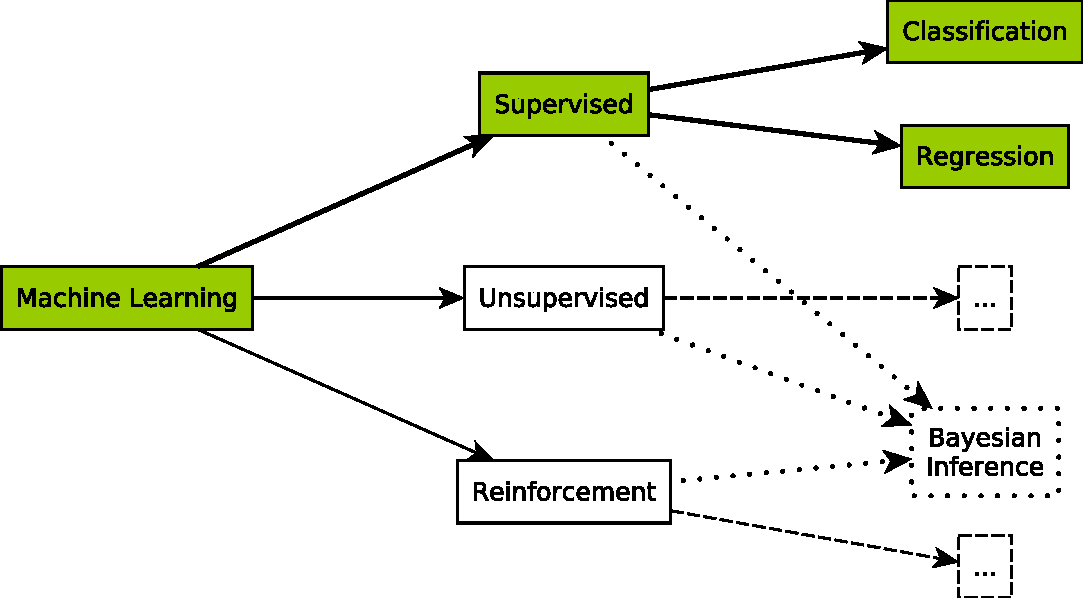
\includegraphics[width=.8\linewidth]{figures/ml-taxonomy.pdf}
    \caption[Taxonomy of ML]{Taxonomy of ML. The second column enumerates the three major families of ML approaches, the third one enumerates the main sorts of tasks affiliated with each family, whereas the fourth one enumerates possible applications for each task.}
    \label{fig:ml-taxonomy}
\end{figure}
%
As depicted in \cref{fig:ml-taxonomy}, three major approaches to ML exist.
%
Each approach is characterised by a well-defined pool of tasks, which may, in turn, be applied in wide range of use case scenarios.
%
The three major approaches to learning are: \emph{supervised}, \emph{unsupervised}, and \emph{reinforcement}.
%
They essentially deal with the kind of task $T$ to be learned -- commonly consisting in the estimation of an unknown relation --, and how expericence $E$ is provided to the learning algorithm.

In supervised learning, the learning task consists of finding a way to approximate an unknown relation, given a sampling of its items---which constitute the experience.
%
In unsupervised learning, the learning task consists of finding the best relation for a sample of items -- which constitute the experience --, following a given optimality criterion intensionally describing the target relation.
%
In reinforcement learning, the learning task consists of letting an agent estimate optimal plans given the reward it receives whenever it reaches particular goals---constituting the experience.
%
There, a plan can be described as a relation among the possible states of the world, the actions to be performed in those states, and the reward the agents expects to receive from that action.

Such categorization of learning approaches can be applied to both symbolic and sub-symbolic techniques.
%
Indeed, in this chapter, we provide an overview of learning on a per repesentation basis.
%
In particular, in the following sections we summarise the state of the art for what concerns both symbolic and sub-symbolic forms of \emph{supervised} learning.

\section{Sub-Symbolic Supervised Machine Learning}

Since several practical AI problems -- such as image recognition, financial and medical decision support systems -- can be reduced to \emph{supervised} ML -- which can be further grouped in terms of either  \emph{classification} or \emph{regression} problems \cite{twala2010,smlreview-faia160} --, in the reminder of this section we focus on this set of ML problems. 

Within the scope of sub-symbolic supervised ML, a \emph{learning algorithm} is commonly exploited to approximate the specific nature and shape of an unknown \emph{prediction} function (or \emph{predictor}) $\pi^*: \mathcal{X} \rightarrow \mathcal{Y}$, mapping data from an input space $\mathcal{X}$ into an output space $\mathcal{Y}$.
%
There, common choices for both $\mathcal{X}$ and $\mathcal{Y}$ are, for instance, the set of vectors, matrices, or tensors of numbers of a given size---hence the sub-symbolic nature of the approach.

An important assumption significantly affecting both the theory and the practice of sub-symbolic supervised learning is that vectors, matrices, or tensors in $\mathcal{X}$ and $\mathcal{Y}$ are of \emph{fixed} size---despite items in $\mathcal{X}$ may have a different sizes than the items in $\mathcal{Y}$.
%
Without lack of generality, in what follows we refer to items in $\mathcal{X}$ as $n$-dimensional vectors denoted as $\mathbf{x}$, whereas items in $\mathcal{Y}$ are $m$-dimensional vectors denoted as $\mathbf{y}$---despite matrices or tensors may be suitable choices as well.

To approximate function $\pi^*$, supervised learning assumes a learning \emph{algorithm} is in place.
%
This algorithm computes the approximation by taking into account a number $N$ of \emph{examples} of the form $(\mathbf{x}_i,\mathbf{y}_i)$ such that $\mathbf{x}_i \in X \subset \mathcal{X}$, $\mathbf{y}_i \in Y \subset \mathcal{Y}$, and $|X| \equiv |Y| \equiv N$.
%
There, the set $D = \{ (\mathbf{x}_i,\mathbf{y}_i) \mid \mathbf{x}_i \in X, \mathbf{y}_i \in Y \}$ is called \emph{training} set, and it consists of $(n+m)$-dimensional vectors.
%
The dataset can be considered as the concatenation of two matrices, namely the $N \times n$ matrix of \emph{input} data ($X$) and the $N \times m$ matrix of \emph{expected output} data ($Y$).
%
There, each $\mathbf{x}_i$ represents an instance of the input data for which the expected output value $\mathbf{y}_i \equiv \pi^*(\mathbf{x}_i)$ is known or has already been estimated.
%
Notably, such sorts of ML problems are said to be ``supervised'' \emph{because} the expected outputs $Y$ are available.
%
Furthermore, the function approximation task is called ``regression'' if the components of $Y$ consist of continuous or numerable -- i.e. \emph{infinite} -- values, or ``classification'' problems they consist of categorical -- i.e. \emph{finite} -- values.

Many learning algorithms exist, and they work in quite different ways.
%
However, the general layout of sub-symbolic supervised learning is the same in all cases.
%
The learning algorithm assumes $\pi^*$ to be a function from a given set of functions $\mathcal{H}$ called \emph{hypotheses} space---i.e. $\pi^* \in \mathcal{H}$.
%
In other words, the underlying assumption is that the unknown prediction function $\pi^*$ exists, and it is of the form characterising all functions in $\mathcal{H}$.
%
The algorithm performs an exploration of the \emph{hypotheses} space $\mathcal{H}$ looking for the hypothesis function $\hat{\pi} \in \mathcal{H}$ that better fits the data in $D$---and that, therefore, better approximates $\pi^*$.

The goodness of the fitting among a hypothesis function $\hat{\pi}$ and the data can be assessed via either 
%
\begin{inlinelist}
    \item an error function $\varepsilon : \mathcal{Y} \times \mathcal{Y} \rightarrow \mathbb{R}_{\geq 0}$ measuring the discrepancy among the expected outputs in $Y$ and the values attained by applying $\hat{\pi}$ to $X$, or dually,
    \item an adherence function $\rho : \mathcal{Y} \times \mathcal{Y} \rightarrow \mathbb{R}_{\leq 1}$, measuring the similarities among the same values.
\end{inlinelist}
%
For the sake of simplicity, we here consider the best hypothesis $\hat{\pi}$ the one item of $\mathcal{H}$ for which the total error is minimal -- or the total adherence is maximal --, w.r.t. the data in $D$. 
%
Therefore, in theory, any sub-symbolic supervised learning process can be abstractly described via any of the following formul\ae{}:
%
$$
\hat{\pi} = \argmin{\pi \in \mathcal{H}}{ \sum_{i=1}^{N} \varepsilon(\mathbf{y}_i,\ \pi(\mathbf{x}_i)) }
\quad \text{or} \quad
\hat{\pi} = \argmax{\pi \in \mathcal{H}}{ \sum_{i=1}^{N} \rho(\mathbf{y}_i,\ \pi(\mathbf{x}_i)) }
$$

\paragraph{Parameters and hyper-parameters}

Exploration of the hypothesis space is what is commonly referred to as ``learning'' or ``training''.
%
Learning algorithms mostly differ for the strategy they follow to perform such exploration, other than the particular hypotheses spaces they support.

A common strategy followed by most learning algorithms leverages on the assumption that the hypothesis space is the set of all functions having the same shape, regulated by a given amount $p$ of \emph{parameters}---namely $\mathcal{H}_\Theta$ where $\Theta \subseteq \mathbb{R}^p$ is space of parameters, enumerated by $\theta$.
%.
Under such assumption, the formulation of supervised learning can be rewritten as the optimisation task of finding the optimal parameters $\theta^*$ among the ones in $\Theta$:
%
$$
\theta^* = \argmin{\theta \in \Theta}{ \sum_{i=1}^{N} \varepsilon(\mathbf{y}_i,\ \pi_\theta(\mathbf{x}_i)) }
\quad \text{or} \quad
\theta^* = \argmax{\theta \in \Theta}{ \sum_{i=1}^{N} \rho(\mathbf{y}_i,\ \pi_\theta(\mathbf{x}_i)) }
$$
%
where $\pi_\theta \in \mathcal{H}_\Theta$ is the particular function using the parameters in $\theta$.

If all functions in $\mathcal{H}_\Theta$, as well as the error (resp. adherence) function $\varepsilon$ (resp. $\rho$), are differentiable w.r.t. $\theta$, then the optimisation task can be tackled via gradient descent (resp. climbing) in the general case---despite better options may exist for particular shapes of the functions in $\mathcal{H}_\Theta$.
%
Such need to rely on differentiable functions of vectors of real numbers is what forces many ML techniques into the sub-symbolic realm.

Notably, a hypothesis space is commonly generated by a particular assignment of a number $q$ of \emph{hyper-parameters} $\omega \in \mathbb{R}^q$.
%
Each particular value of $\omega$ corresponds to a particular parameters space $\Theta$, and therefore to a particular hypothesis space $\mathcal{H}_\Theta^\omega$.
%
The hypothesis space may consist for instance of the set of all polynomials of $a$ variables whose degree is $b$.
%
That would imply the corresponding parameters space to comprehend all possible vectors having $\binom{b}{a}$ components.
%
So, if $a = b = 1$, then $\mathcal{H}_\Theta^\omega$ is the set of all possible straight lines on a plane, i.e. polynomials parametrised by $\theta_1$ and $\theta_2$.
%
For $a = 1$ and $b = 2$, $\mathcal{H}_\Theta^\omega$ corresponds to the set of all possible parabolas on a plane, i.e. polynomials parametrised by $\theta_1$ and $\theta_2$ and $\theta_3$.
%
A similar example may be built upon polynomials of 2 variables, and so on.

The difference among parameters and \emph{hyper-}parameters is very important in practice.
%
In fact, while parameters are \emph{automatically} computed by the learning algorithm, hyper-parameters are not.
%
They may be either guessed or estimated by trial-and-error by data scientists---hence representing a bottleneck in the automatisation of learning. 

\note{About generalisation: the bias-variance trade-off?} % maybe out of topic

\note{Comments on the role of feature engineering} % already discussed in chap on KR

\subsection{Overview on learning algorithms}

\note{
    Comments on existing algorithms and their relevant aspects?
    Let's distinguish among parametric and non-parametric algorithms.
    Let's distriguish among regression and classification algorithms, with a focus on regression as classification can be reduced to regression.
    Focus on gradient descent, backpropagation and deep learning.
}

% Depending on the predictor family $\mathcal{P}$ of choice, the nature of the learning algorithm and the admissible shapes of $\hat{p}$ may vary dramatically, as well as the their \emph{interpretability}.
% %
% Even if the interpretability of predictor families is not a well-defined feature, most authors agree on the fact that some predictor families are \emph{more interpretable than others} \cite{Lipton18}---in the sense that it is easier for humans to understand the functioning and the predictions of the former ones.
% %
% For instance, it is widely acknowledged that \emph{generalized linear models} (GLM) are more interpretable than neural networks (NN), whereas \emph{decision trees} (DT) \cite{breiman1984classification} are among the most interpretable families \cite{GuidottiMRTGP19}.

\section{Symbolic Supervised Learning}

Within the realm of symbolic AI, supervised ML commonly refers to either \emph{inductive logic programming} (ILP) \cite{Muggleton91} or \emph{statistical relational learning} (SRL) \cite{DeRaedt2010}, despite the overlap among the two disciplines is wide.

In both cases, learning consists of approximating an unknown \emph{intensional} representation $H^*$ for a number of positive examples $E^+$, possibly leveraging on 
%
\begin{itemize}
    \item some prior KB $B$, carrying the so-called \emph{background knowledge} about the domain at hand;
    \item a number of \emph{negative} examples $E^-$;
    \item a \emph{language bias} $C$, constraining the admissible shapes for the representation to-be-learned.
\end{itemize}
%
In the general case, $H^*$, $E^+$, $E^-$, and $B$ are knowledge bases, possibly involving several definite clauses (i.e. either rules or facts), while the shape of $C$ really depends on the particular learning approach at hand. 
%
Of course, there may be cases where $E^-$, $B$ or $C$ are not required, and therefore considered as empty sets.

The main difference among ILP and SLR lays in the particular language used for knowledge representation.
%
While in ILP knowledge bases simply consist of bare definite clauses, SRL leverages on a superset of Horn Logic called ProbLog \cite{RaedtKT07}, where definite clauses are enriched with probability values.

According to the SLR nomenclature of \cite{DeRaedt2010} -- where a unifying model generalising ILP and SLR is proposed --, there are two relevant problems which lay under the symbolic supervised learning umbrella, namely:
%
\begin{description}
    \item[parameters learning] where $H$ consists of a given ProbLog KB, where the shape of facts and rules is known, while their probabilities are not, and learning aims at simply estimating those probabilities
     
    \item[structure learning] where $H$ is completely unknown, and the whole shape of facts and rules therein contained must be computed, possibly along with their corresponding probabilities 
\end{description}

In both cases, learning can be defined as an optimisation problem aimed at approximating $H^*$ by search for the best KB $\hat{H}$ into an hypothesis space $\mathcal{H}_{B,C}$, defined by applying all possible combinations of clauses in $B$, as dictated by $C$.
%
There, each KB $H \in \mathcal{H}_{B,C}$ consists of a number of definite clauses defining the $n$-ary relation $h$, possibly leveraging on the relations defined in $B$, and satisfying the suggestions/constraints expressed by $C$.
%
In other words, they consist of KB intensionally defining $h$ via rules of the form:
%
\begin{equation*}
    \psi :: h(X_1,\ \ldots,\ X_n) \leftarrow f(\bar{X}),\ f'(\bar{X}'),\ f''(\bar{X}''),\ \ldots
\end{equation*} 
%
where $\psi$ denotes an optional probability value,  while $\bar{X}, \bar{X}', \bar{X}'', \ldots$ are tuples involving one or more head variables (i.e., $X_1, \ldots, X_n$), and $f, f', f'', \ldots$ are either predicates defined in $B$ or combinations of those predicates, attained by following the suggestions/constraints contained in $C$.
%
Similarly, $E^+$ (resp. $E^-$) consists of facts of the form $h/n$, extensionally defining known (resp. invalid) items of the $n$-aray relation $h$, and possibly labelled with probabilities.

Analogously to the sub-symbolic case, symbolic supervised learning leverages upon some adherence function $\rho$, aimed at measuring the adherence of some hypothesis KB $H \in \mathcal{H}_{B,C}$ w.r.t. either $E^+$ or $E^-$.
%
For instance, in SRL, $\rho$ is commonly modelled probabilistically:
%
\begin{equation*}
    \rho(H, E, B) = \sum_{e \in E} \mathbb{P}(e \mid H, B)
\end{equation*}
%
where $\mathbb{P}(\cdot \mid \cdot)$ denotes the conditional probability operator.
%
Conversely, in ILP, $\rho$ is modelled in terms of logic inference\footnotemark:
%
\begin{equation*}
    \rho(H, E, B) = \sum_{e \in E} \rho(H, e, B)
    \quad \text{and} \quad
    \rho(H, e, B) = \begin{cases}
        1 & \text{if} ~ H, B \models e 
        \\
        0 & \text{otherwise} 
    \end{cases} 
\end{equation*}
%
\footnotetext{
    This aspect is better discussed in \cref{chap:reasoning}. 
    %
    Within the scope of this chapter, the notation $K \models \phi$, where $K$ is a knowledge base and $\phi$ is a logic formula, can simply be read as ``$\phi$ can be inferred from $K$ via some inference procedure''.
}
%
Under such hypothesis, symbolic supervised learning can be defined as \cite{DeRaedt2010} the optimisation task aimed at finding the hypothesis which adheres to as much positive examples as possible, while adhering to no negative example at all:
%
\begin{equation}
    \hat{H} = \argmax{H \in \mathcal{H}_{B,C} ~ \text{s.t.} ~ \rho(H, E^-, B) = 0}{\rho(H, E^+, B)}
\end{equation}

Parameter and structure learning differ for the actual way the search is performed, other than for the actual object of search.
%
In parameter learning, algorithms can assume the shape of (facts and rules in) $\hat{H}$ to be given (and fixed), and therefore focus on the mere esitmation of probabilities.
%
Conversely, in structure learning, algorithms must also consider the many possible shapes $\hat{H}$ may have.
%
This includes all possible combinations of all relations possibly defined in $B$.
%
Assuming, for instance, that $B$ intensionally defines $r$ relations $f_1, \ldots, f_r$, whose arity is at least $a$, and that the target relation is $h$, whose arity is $n$.
%
Under such hypothesis, rules in $H$ should be of the form:
%
\begin{equation*}
    h(X_1,\ \ldots,\ X_n) \leftarrow \ldots
\end{equation*} 
%
where the body of the rule may contain as many predicates as in any possible permutation of any possible subset of $\{ f_1, \ldots, f_r \}$.
%
There, each possible $a$-ary relation could be written as a predicate involving some disposition of $a$ variables from the set $\{ X_1, \ldots, X_n \}$.
%
In other words, the search space for structure learning is \emph{huge} and definitely impossible to explore in useful time, unless in trivial cases.
%
To complicate the matter, differently from the sub-symbolic case, the search space is not even continuous---meaning that gradient based approaches cannot be applied.

To mitigate such issues -- and to reduce the search space --, the ILP community leverages on smart choices of the linguistic bias $C$.
%
The general purpose of the linguistic bias is to constrain the particular way relations from $B$ can be combined in $H$.
%
For instance, in the meta-interpretative learning approach \cite{MuggletonLPT14}, $C$ consists of a library of higher-order rules (a.k.a. meta-rules), which define the admissible sorts of combinations.
%
There, a meta-rule is a rule involving higher-order variables enumerating over predicate symbols, such as:
%
\begin{equation}\label{eq:meta-rule-example}
    \textsf{P}(A,\ B) \leftarrow \textsf{Q}(A,\ C),\ \textsf{R}(C,\ B) 
\end{equation}
%
where uppercase, sans-serif letters $\textsf{P}, \textsf{Q}, \textsf{R}$ denote higher-order variables, while $A, B, C$ are ordinary variables; and the whole formula allows an induction algorithm to \emph{invent} \cite{MuggletonB88} some binary predicate $\textsf{P}$ by combinations of two binary predicates $\textsf{Q}$ and $\textsf{R}$.

Consider for instance the case of an ILP problem aimed at learning the positive example $grandparent(\functor{abraham}, \functor{jacob})$, given the background knowledge containing a number of facts expressing parenthood facts of the form $parent(\functor{p}, \functor{p}')$, describing Abraham's family tree---as in \cref{eq:abraham-family-tree}.
%
There, the meta-rule \ref{eq:meta-rule-example} may suggest the correct identification of the target rule -- namely, $grandparent(X, Y) \leftarrow parent(X, Z), parent(Z, Y)$ -- via the variable assignment $\{ \textsf{P} \mapsto grandparent, \textsf{Q} \mapsto parent, \textsf{R} \mapsto parent \}$.

It is worth to be noted how the language bias $C$ plays, in symbolic supervised learning, the same role played by hyper-parameters in sub-symbolic supervised learning.
%
In both cases, \emph{automated} learning relies on some prior knowledge, which must be handcrafted by data scientists.
%
In fact, similarly to sub-symbolic approaches, some mechanism is needed to let humans control either the complexity or learning or the dimension of the search space.
%
In the particular case of symbolic supervised learning, that mechanism is the language bias.

\subsection{Overview on learning algorithms}

\note{
    Intuition behind the functioning of the algorithms.
    ProbLog as the main approach to SRL.
    Bottom up or top down approaces in ILP.
    Mention main approaches: relatively least general generalisation, reverse entailment, bottom clause generalisation, meta-interpretative learning.
    Mention major algorithms developed in this field.    
}

\section{Symbolic vs. Sub-Symbolic Learning}

Symbolic and sub-symbolic approaches to supervised learning share similar formulations, despite the corresponding methods and algorithms operate in quite different ways.
%
Both formulations deal with optimisation problems aimed at iteratively construting an algorithm mimicking an unknown relation/function in the best possible way, leveraging on a number of examples.
%
However, because of their nature and the inherent way they represent knowledge, both approaches come with pros and cons.
%
Here we focus, on their flexibility, maturity, data and computational efficiency, degree of automation, and validation.

\paragraph{Flexibility and maturity}

For what concerns flexibility, symbolic approaches produce more flexible outcomes, whereas sub-symbolic approaches are characterised by more flexible learning processes.

\subparagraph{Outcomes}

Focussing on symbolic approaches, flexibility lays in the shape of the expected outcomes, which is a direct effect of the particular choice of symbols for KR.
%
``Symbolic'' here implies that knowledge is represented via logic clauses, which in turn pave the way towards learning intensional \emph{relations}---possibly taking some prior (background) knowledge into account.
%
Indeed, representing the target of knowledge in the form of relations expressed by logic formul\ae{} comes with two major advantages---namely bi-directionality and re-usability.

First, relations are \emph{bi-directional}, meaning that any argument of the relation can be considered either an input or an output, depending on the situation at hand.
%
So, for instance, if an agent is capable of learning the clauses expressing the $grandparent/2$ relation -- cf. \cref{eq:abraham-family-tree} --, then it acquires a lot of relevant information, namely:
%
\begin{inlinelist}
    \item an explicit, generic representation of \emph{how} the relation can be tested among any two entities $X$ and $Y$,
    \item a way to compute all the grand-children of any given grand-parent $\functor{p}$ -- i.e. $grandparent(\functor{p}, Y)$ --, and
    \item a way to compute all the grand-parents of any given grand-child $\functor{c}$---i.e. $grandparent(X, \functor{c})$.
\end{inlinelist}

Second, relations are \emph{re-usable} (w.r.t. a learning process), meaning that learned relations can be used as prior knowledge in any sub-sequent learning process, as both the inputs and outputs of any symbolic learning process are represented in the same form---namely, logic clauses.
%
This in turn paves the way towards the definition of learning \emph{cycles} where a learning algorithm is executed several times and the knowledge acquired after each round is included in the background knowledge of successive rounds.

Conversely, sub-symbolic approaches aim to learn \emph{functions}, rather than relations.
%
The learned functions are generally \emph{mono-directional} -- in the sense that they are not (easily) invertible -- and extensional.
%
Consider for instance the case of a neural network aimed at classifying images of animals.
%
It may easily discriminate among dogs and cats (i.e. compute the classification, given an input), yet it may hardly generate admissible images of neither dogs or cats (i.e. compute an input, given a class)\footnotemark.

\footnotetext{Generative Adversarial Neural Networks \cite{GoodfellowPMXWOCB14} may be used whenever bi-directionality is needed, yet that essentially implies traning two networks: one \emph{classifier} and one \emph{generator} of data, where the former can only classify, and the latter can only generate data.}

\subparagraph{Processes}

Focussing on sub-symbolic approaches, flexibility lays in the variety of methods to approximate the target function.
%
Such variety is once again the result of the particular choice of arrays of numbers for KR.
%
In fact, this choice enables the pervasive exploitation of mathematical operations as the basic bricks of sub-subolic processing. %learning and computing.
%
These include basic algebraic operators (sum, product, etc.), as well as statistical (mean, variance, standard deviation, etc.), information-theoretical (cross-entropy, mutual information, etc.), signal-processing (Fourier- or Laplace-transform, etc.), binary (bitwise-and, -or, etc.), or differential (differentiation, integration, etc.) operators.
%
All such operators, in turn, come with two major advantages in terms of \emph{malleability} and \emph{parallelisation}.

Malleability refers to the capability of learning in spite of how the many elementary operators are combined.
%
Within the scope of sub-symbolic approaches, malleability is commonly guaranteed by the pervasive exploitation of \emph{differentiable} operators, which supports learning via numeric optimisation algorithms---e.g. stochastic gradient descent (SGD) and its variants \cite{enwiki:SGD}.
%
Conversely, within the scope of symbolic approaches, the presence (resp. lack) of any given operator may greatly affect the \emph{expressiveness} of the underlying logic, therefore making learning more (resp. less) complex from a computational perspective.

Parallelisation refers to the capability of speeding up learning algorithms by executing as much sub-tasks as possible in parallel, provided that the adequate hardware is in place.
%
Within the scope of sub-symbolic approaches, most basic methematical operators -- such as matrix- or tensor-products --, as well as whole learning steps -- such as \emph{batches} in SGD --, can be executed in parallel to some extent, possible via ad-hoc hardware facilities
%
Conversely, within the scope of symbolic learning, futher research on concurrent / parallel solutions is still needed.

Consider, for instance, neural networks as opposed to ILP.
%
They are characterised by a great flexibility because of their reliance on differentiable operators (mostly sums, multiplications and activation functions \cite{enwiki:ActivationFunctions}), and malleable way of combining them into arbitrarly complex structures.
%
Therefore, regardless of the complexity of the overall structrure, a NN is composed by the recursive composition of differentiable operators---which makes the whole network trainable via SGD.
%
To further speed up NN training, a plethora of software frameworks have been designed and implemented, with the purpose of exploiting ad-hoc hardware, such as GPUs---cf. Tensorflow, Theano, Caffe, etc. \missingref.
%
Conversely, despite the many algorithms designed for ILP, the avilability of software frameworks reifying them is quite scarce, and the support for parallelisation is even scarcer.
%
Should we speculate on the motivations behind this situation, we would argue that symbolic and sub-symbolic approaches to learning have so far reached different levels of \emph{maturity}---expecially, for what concerns technological readiness.

% \note{Higher flexibility of symbolic learning which learns intensional representations, yet higher maturity of sub-symbolic approaches.}

\paragraph{Efficiency}

Efficiency in learning can be measured against two major aspects, namely time and space.
%
Data (resp. computational) efficiency deals with space (resp. time), and it is related to the amount of data (resp. time) required by learning to be effective.
%
% Computational efficiency deals with time, and it is related the amount of time required by learning to be effective.
%
% In both cases, 
Here, effectivess refers to the adherence of the learned relation/function w.r.t. the available examples.

Concerning data efficiency, sub-symbolic approaches are notably data-hungry \cite{Adadi21}, as they require tons of examples to learn tasks for which a human would require just a handful.
%
Conversely, symbolic approaches are considered far more data-efficient.
%
In \cite{EvansG18}, the authors discuss this notable difference, arguing that a motivation may lay in the strong language bias imposed by choice of logic formul\ae{} as the preferred means for KR.

Concerning computational efficiency, while in theory both symbolic and sub-symbolic approaches must explore \emph{infinite} search spaces, in practice, efficiency can be improved by 
%
\begin{inlinelist}
    \item sacrificying effectivess, e.g. by leveraging on greedy algorithms, strong biases, or aggressive stopping criteria,
    \item parallelising the learning algorithm, as discussed above.
\end{inlinelist}

% \note{Data efficiency: sub-symbolic approaches usually require more data. Computational efficiency: sub-symbolic approaches can be parallelised, especially GD, eg. via GPUs. Symbolic approaches cannot}.

\paragraph{Automation and autonomy}

% \note{Similar formulation, similar issue: no silver bullet, i.e. not everthing is handled automatically}

A commond trait shared by both symbolic and sub-symbolic approaches to supervised learning is their reliance on semi-automatic workflows.
%
In other words, despite the name, both apporaches require a ``human in the loop'' -- namely, the data scientist -- to take care of those aspects which learning algorithms cannot autonomously deal with.
%
In the case of sub-symbolic approaches, these aspects involve the choice of hyper-parameters.
%
In the case of symbolic approaches, these aspects involve the choice of the language bias and background knowledge.
%
In both cases, these aspects involve the choice of the most adequate learning algorithm(s), other than the engineering of the representation of available data, in maximise the effectiveness the learning algorithm(s).

Within the scope of sub-symbolic learning, the problem of hyper-parameters tuning is currently addressed via a number of practices aimed at automating and speeding up their selection.
%
A summary of such practices can be found in \cite{ClaesenM15}.
%
The recent advances in the field of \emph{Automated ML} \cite{HeZC21} are building on such practices in order to further increase the degree of automation in sub-symbolic ML.
%
However, current efforts are focussing on supporing data-scientists in an end-to-end fashion, rather than letting software agents learn autonomously.

To the best of our knowledge, automating the definition of background knowledges and language biases in symbolic learning is not a major concern.
%
Should we speculate on the reasons behind this phenomenon, we would argue that both background knowledges and language biases are the preferred way to let human beings tranfer their commonsense and winsdowm to the learning algorithms.
%
In this sense, the creation of background knowledges and language biases is inherently poorly automatable.
%
However, background knowledges can be incrementally constructed by an agent (be it human or software) and then shared or transferred to other agents.
%
A similar argument may hold for language bias, since it may be consideres as meta-level background knowledge---i.e. knowledge about how further knowledge may be constructed.

% \paragraph{Validation}

% \note{Sub-symbolic approaches care a lot about model validation as a means to assess the generalisation capabilities of a trained model. ILP model care less. Speculating on the motivation: the outcome of ILP is symbolic, therefore the human being can understand if it is correct or not. Or maybe it's simply because it has not been applied on a large scale, yet?}

\chapter{Reasoning over Knowledge}\label{chap:reasoning}

The Cambridge dictionary\footnote{\url{https://dictionary.cambridge.org/it/dizionario/inglese/reasoning}} defines \emph{reasoning} as 
%
``the process of thinking about something in order to make a decision''.
%
Conversely, the Oxford dictionary\footnote{\url{https://www.oxfordlearnersdictionaries.com/definition/english/reasoning?q=reasoning}} states that reasoning is 
%
``the process of thinking about things in a logical way''.
%
Notably, while both definitions agree that reasoning essentially consists in the \emph{process of thinking}, none of them actually constrains the nature of the entity enacting this process, despite thinking -- and, in particular, reasoning -- is the most characterising capability of \emph{humans}' mind.
%
This welcomes the idea that software agents may be capable of \emph{automated} reasoning as well.

Indeed, within the scope of this thesis, we consider reasoning as the activity performed by an agent (either human, or computational) whenever it draws new knowledge out of prior knowledge.
%
Of course, as for learning, the particular way knowledge is drawn heavily depends on how it is represented.

When knowledge is symbolically represented, reasoning leverages on one or more \emph{inference rules}, i.e. logic formul\ae{} dictating under which conditions conclusions may be draw out of premises.
%
This reflects the Oxford definition, where the \emph{logic} nature of reasoning is stressed.
%
Inference rules may be used, for instance, to deduce a particular case from a general rule, to induce the general rule justifying a number of observations, or to speculate on the possible causes for some phenomena, given the particular rules governing the underlying noumena.
%
Therefore, within the symbolic realm, the terms ``inference'' and ``reasoning'' are used almost interchangeably.
%
% Under such setting, when it comes 
Research in this field aims at letting computational agents draw logic inferences automatically.
%
For this reason, the focus of computer scientists is on finding effective and efficient algorithms to let agents reason autonomosly---i.e. with minimal human intervention.

Conversely, when knowledge is sub-symbolically represented, ``inference'' and ``reasoning'' are \emph{reduced} to the data-analytic activity of applying the models learned from previous data to novel data, in order to mine useful information.
%
Such activity is far from trivial, as it may used to perform tasks which would be prohibitively complex to express otherwise---e.g. image recognition.
%
Accordigly, the Cambridge definition is more adequate in this case: reasoning is not necessarily logic in nature, but for sure it is aimed at driving decisions---e.g. deciding whether handwritten characted is more likely a 1 or a 7, or whether an histological image should or should not raise an alarm for cancer.
%
Research in this field aims at letting sub-symbolic algorithms attain better predictive performances.
%
As such, data scientists' efforts are mostly devoted to the improvement of \emph{learning} algorithms, as inference is straightworard.
%
However, recent research efforts are being devoted to the exploitation of sub-symbolic algorithms as means for performing symbolic computations---therefore mimicking logic reasoning.

In the reminder of this chapter we delve into the details of reasoning from both a symbolic and sub-symbolic perspective.
%
In particular, we present the classic approaches and algorithms to automate logical reasoning and we introduce the theory behind the mimicking of symbolic reasoning via sub-symbolic facilities.

\section{Symbolic Reasoning}
\mypapers{logictech-information11}

Symbolic (i.e., logic-based) reasoning approaches root back to John McCarthy's work of 1958 \cite{Mccarthy1958}, aimed at developing the idea of formalising the so-called \emph{commonsense reasoning} to build intelligent artefacts---i.e. computational or cyber-physical agents endowed with human-like intelligence.
%
There, commonsense intuitively refers to the basic understanding of the physical world, its cause-effect rules, and the effects of one's actions on it, etc \cite{Mccarthy1989}.
%
It is such an obvious capability for human beings that most of it is not even explicitly taught in schools, yet it is incredibly hard to formalise and represent for computational agents, which are therefore inherently lacking such kind of basic knowledge.

Despite the formalisation of commonsense soon proved to be very challenging -- mostly because of the many non-trivial involved issues, such as the need of formalising the situation the agent is immersed into, actions it may perform of be subject to, and physical and legal laws govering its environment and context, etc. --, many frameworks and tools have been developed over the years while pursuing such goal.
%
There are freely available commonsense knowledge bases and natural language processing toolkits, supporting practical textual-reasoning tasks on real-world documents including analogy-making, and other context oriented inferences---see for instance \cite{lieberman2004,trinh2018,liu2004conceptnet,liu2002goose,shapiro1999sneps}). \missingref
%
There have been also a number of attempts to construct very large knowledge bases of commonsense knowledge by hand, one of the largest being the CYC program by Douglas Lenat at CyCorp \cite{lenat1995-cyc}. \missingref

The modern approach to automated reasoning starts with Robinson's resolution principle \cite{robinson1965}: since then, several technologies have exploited \emph{deduction} on FOL knowledge bases to provide reasoning capabilities in diverse areas---logic programming, deductive data bases, and constraint logic programming (CLP) possibly being the major ones.
%
Other approaches and techniques, however, built upon the \emph{induction} and \emph{abduction} principles.

As its name suggests, \emph{deduction} operates top-down, deriving a true conclusion from a universal true premise: logically speaking, this means that the conclusion's truth necessarily follows from the premise's truth.
%
\emph{Induction}, instead, operates bottom-up, basically making a guess -- a generalization -- from specific known facts: so, the reasoning involves an element of probability, as the conclusion is not based on universal premises.
%
\emph{Abduction} is somehow similar, but seeks for cause-effect relationships---i.e., the goal is to find out under which hypotheses (or premises) a certain goal is provable. 
%
Such technologies are exploited, in particular, for the verification of compliance of specific properties \cite{montali2010}. 

\emph{Logic programming} (LP) is likely the most widely-adopted paradigm based on deduction. 
%
From Colmerauer and Kowalsky's seminal work \cite{Kowalski1974,colmerauer1986-theoreticalProlog}, the Prolog language has been since then one of the most exploited language in AI applications \cite{Dawson1996}. 
%
Other valuable approaches include \emph{fuzzy logic}, \emph{answer-set programming} (ASP), \emph{constraint logic programming} (CLP), \emph{non-monotonic reasoning}, and \emph{belief-desire-intention} (BDI).

Fuzzy logic \cite{yen1999} aims at dealing with lack of precision or uncertainty.
%
In this sense, it is perhaps closer in spirit to the human thinking than traditional logic systems. 
%
Not surprisingly, fuzzy approaches are exploited as a key technology in specific application areas, e.g., the selection of manufacturing technologies \cite{goyal2012}, and industrial processes where the control via conventional methods suffers from the lack of quantitative data about I/O relations.
%
There, a fuzzy logic controller effectively synthesises an automatic control strategy from a linguistic control strategy based on an expert's knowledge. 

\emph{Answer set programming} (ASP) and \emph{constraint logic programming} (CLP) are the two main logical paradigms for dealing with various classes of NP-complete combinatorial problems. 
%
ASP solvers are aimed at computing the answer sets of standard logic programs; these tools can be seen as theorem provers, or model builders, enhanced with several built-in heuristics to guide the exploration of the solution space.
%
% Some of the best known solvers are Clingo \cite{gebser2014-clingo} and DLV \cite{eiter2000}.

Constraint logic programming (CLP) \cite{jaffar1987}, perhaps the most natural extension of LP (or, its most relevant generalisation), has evolved over the years into a powerful programming paradigm, widely used to model and solve hard real-life problems \cite{Rossi2000} in diverse application domains---from circuit verification to scheduling, resource allocation, timetabling, control systems, etc.
%
CLP technologies can be seen as complementary to \emph{operation research} (OR) techniques: while OR is often the only way to find the optimal solution, CLP provides generality, together with a high-level modelling environment, search control, compactness of the problem representation, constraint propagation, and fast methods to achieve a valuable solution \cite{rossi2008}.
%
% CLP tools evolved from the  ancestor -- CHIP \cite{simonis1995-chip}, the first to adopt constraint propagation -- to the constraint-handling libraries of ILOG \cite{ilog} and COSYTEC \cite{aggoun1993}, up to CLP languages such as Prolog III \cite{colmerauer1990}, Prolog IV \cite{benhamou1995}, CLP(R) \cite{jaffar1992}, and clp(fd) \cite{codognet1996}.

Non-monotonic reasoning means to face the basic objection \cite{minsky1975} that logic could not represent knowledge and commonsense reasoning as humans because the human reasoning is inherently \emph{non monotonic}---that is, consequences are not always preserved, in contrast to first-order logic.
%
Since then, a family of approaches have been developed to suit specific needs---among these, \emph{default reasoning} \cite{reiter1980}, \emph{defeasible reasoning} \cite{pollock1987}, \emph{abstract argumentation} theory \cite{bondarenko1997}. 
%
Defeasible reasoning, in particular, is widely adopted in \emph{AI \& law} applications, to represent the complex intertwining of legal norms, often overlapping among each other, possibly from different, non-coherent sources.
%
Abstract argumentation theory, in its turn, is concerned with the formalisation and implementation of methods for rationally resolving disagreements, providing a general approach for modelling conflicts between arguments, and a semantics to establish if an argument can be acceptable or not.

Belief-desire-intention (BDI) logic is a kind of modal logic used for formalising, validating, and designing cognitive \emph{agents}---typically, in the \emph{multi-agent systems} (MAS) context.
%
A cognitive agent is an entity consisting of 
%
\begin{inlinelist}
    \item a belief base storing the agent's \emph{beliefs}, i.e. what the agent knows about the world, itself, and other agents;
    \item a set of \emph{desires} (or goals), i.e. the proprieties of the world the agent wants to eventually become true;
    \item a \emph{plan} library, encapsulating the agent's procedural knowledge (in the form of plans) aimed at making some goals become true; and
    \item a set of \emph{intentions}, storing the states of the plans the agent is currently enacting as an attempt to satisfy some desires.
\end{inlinelist}
%
All such data usually consist of first-order formulas.
%
Then, the dynamic behaviour of a BDI agent is driven by either internal (updates to the belief-base or changes in the set of desires) or external (perceptions or messages coming from the outside) events, which may cause new intentions to be created, or current intentions to be dropped.
%
By suitably capturing the revision of beliefs, and supporting the concurrent execution of goal-oriented computations, BDI architectures overcome critical issues of ``classical'' logic-based technologies -- \emph{concurrency} and \emph{mutability} -- in a sound way.
%
Overall, BDI architecture leads to a clear and intuitive design, where the underlying BDI logic provides for the formal background.
%
Among the frameworks rooted on a BDI approach, let us mention the AgentSpeak(L) \cite{Rao96} abstract language and its major implementation, namely Jason, Structured Circuit Semantics \cite{lee1994}, Act Plan Interlingua \cite{huber1999-jam}, JACK \cite{howden2001}, and dMARS---a platform for building complex, distributed, time-critical systems in C++ \cite{dmars}.

In the reminder of this section we focus on logic programming as the most common means to endow computational agent with reasoning capabilities.
%
Before doing so, however, we recall major definitions and notations concerning logic inference as a means for manipulating knowledge.

\subsection{Symbolic Inference} % Deduction, Abduction, Induction, Probabilistic, etc.

% Inference as the operation of producing new knowledge by applying rules to knowledge base.
Within the realm of symbolic AI and, in particular, computational logic, inference is the process of mechanically producing new knowledge by applying rules to some knowledge base.
%
Such rules are commonly expressed via a particular notation, heavily leveraging on the notion of \emph{unification}.

\paragraph{Substitutions and Unification}

Unification \cite{MartelliMontanari1982} is among the most fundamental mechanism in CL: it enables the formalisation of inference, as well virtually any other symbolic manipulation of logic formul\ae{}.

Informally speaking, unification aims at computing a \emph{unifier} among any two FOL formul\ae{}, i.e. a substitution (a.k.a. assignments of variables) making the two formul\ae{} syntatically equal, by properly assigning the variables therein contained.
%
So, in other words, unification computes substitutions out of logic formul\ae{}, checking whether they can be made equal, or failing otherwise.

We denote substitutions as sets of mappings of the form $\sigma = \{ X \mapsto \phi, X' \mapsto \phi', X'' \mapsto \phi'', \ldots \}$, where $X, X', X''$ are variables, and $\phi, \phi', \phi''$ are FOL formul\ae{}.
%
Furthermore, we enumerate substitutions by $\sigma$ or $\omega$.
%
Finally, we let the binary operator $(\cdot)$ denote the application of a substitution to either a formula or another substitution.
%
So, for instance $\phi \cdot \sigma$ denotes the formula attained by applying all variable assignments carried by $\sigma$ to $\phi$.
%
Similarly, $\sigma \cdot \omega$ denotes the substitution attained by applying $\omega$ to the right-hand-side of all variable assignments in $\sigma$.

Consider for instance the case of the general clause $\phi$ and its particular case $\psi$
%
\begin{equation*}
    \begin{array}{c}
        \phi \equiv (g(X, Y) \leftarrow f(X, Z), f(Z, Y))
        \\
        \psi \equiv (g(\functor{a}, \functor{b}) \leftarrow f(\functor{a}, \functor{c}), f(\functor{c}, \functor{b}))
    \end{array}
\end{equation*}
%
The two clauses can be made syntactically equal via the substitution $\sigma = \{ X \mapsto \functor{a}, Y \mapsto \functor{b}, Z \mapsto \functor{c} \}$, because $\psi = \phi \cdot \sigma$.

Accordingly, a unifier among any two non-ground FOL formul\ae{} $\phi$ and $\psi$, is defined as a substitution $\sigma$ such that $\phi = \psi \cdot \sigma$.
%
A trivial way to recursively compute a unifier among $\phi$ and $\psi$ is as follows:
%
\begin{equation}
    \unify{\phi}{\psi} = \begin{cases}
        \varnothing & \text{if} ~ \phi = \psi = \functor{x}
        \\
        \{ X \mapsto Y \} & \text{if} ~ \phi = X \wedge \psi = Y
        \\
        \bigcup_{i}^{N} \unify{\alpha_i}{\alpha'_i} & \text{if} ~ \phi = f(\alpha_1, \ldots, \alpha_N) 
        \\
        & \qquad \wedge\ \psi = f(\alpha'_1, \ldots, \alpha'_N)
        \\
        \unify{\alpha_1}{\alpha'_1} \cup \unify{\alpha_2}{\alpha'_2}  & \text{if} ~ \phi = \alpha_1 \odot \alpha_2 \wedge \psi = \alpha'_1 \odot \alpha'_2
        \\
        \square & \text{otherwise}
    \end{cases}
\end{equation}
%
where $\square$ denotes the lack of any unifier -- capturing the situation where two formul\ae{} cannot be unified -- and $\varnothing$ denotes the empty substitution -- characterising the situation where two formul\ae{} are identical.
%
There, $f$ is either a predicate or functor symbol ($N$-ary, in both cases), $\alpha_i, \alpha'_i$ are arbitrary formul\ae{}, and $\odot$ denotes any binary logical connective.

More precisely, unification aims at computing the \emph{most general} unifier (MGU), i.e. the unifier $\sigma^*$ such that, for each subsitution $\sigma$ making $\phi$ and $\psi$ syntactically equal (i.e., $\phi = \psi \cdot \sigma$) there exists a substitution $\omega$ making it possible to write $\sigma$ as a particular case of $\sigma^*$ (i.e., $\sigma = \sigma^* \cdot \omega$).
%
Despite computing the MGU among any two formul\ae{} is a non-trivial problem in general, an efficient algorithm is describen in \cite{MartelliMontanari1982}.
%
A formal description of this algorithm lays outside this chapter.
%
However, in what follows we denote by $\mgu{\phi}{\psi}$ the function computing the MGU among any two FOL formul\ae{}.

\paragraph{Inference Rules}

Inference rules are functions mapping premises (logic formul\ae{}) into conclusions (other logic formul\ae{}).
% 
They can be denoted both as $\phi_1, \ldots, \phi_N \vdash \psi_1, \ldots, \psi_M$ or as 
%
\begin{equation*}
    \frac{\phi_1, \ldots, \phi_N}{\psi_1, \ldots, \psi_M} ~ [\text{Rule name}]
\end{equation*}
%
where $\phi_1, \ldots, \phi_N$ are premises and $\psi_1, \ldots, \psi_M$ are conclusions.
%
Both expressions can be read as ``when all $\phi_1, \ldots, \phi_N$ are known to hold, then all $\psi_1, \ldots, \psi_M$ can be inferred''.

The notation if often abused by only including among the premises those formul\ae{} which are strictly needed to draw conclusions.
%
When this is the case, a knowledge base $\mathbf{K}$ is then assumed, behind the scenes.
%
Thus, rules of the form $\phi \vdash \psi$ are usually written as concise notation for $\exists \sigma$ s.t. $\phi \cdot \sigma \in \mathbf{K} \vdash \psi \cdot \sigma$.

A plethora of inference rules have been defined in the history of logic.
%
Here we focus on four major examples, correspoding to as many inference principles, namely: 
%
\begin{equation*}
    \frac{\alpha \rightarrow \beta, \alpha}{\beta} ~ [\text{Modus Ponens}]
    \qquad
    \frac{\phi\cdot\sigma_1, \ldots, \phi\cdot\sigma_n}{\phi} ~ [\text{Subsumption}]
\end{equation*}
\begin{equation*}   
    \frac{\alpha \rightarrow \beta, \lnot\beta}{\lnot\alpha} ~ [\text{Modus Tollens}]
    \qquad
    \frac{\alpha \rightarrow \beta, \beta}{\alpha} ~ [\text{Abduction}]
\end{equation*}

Modus ponens (resp. tollens) is a \emph{deductive} inference rule, stating that whenever one knows that $\alpha$ implies $\beta$ and $\alpha$ is true (resp. $\beta$ is false), then they can infer $\beta$ (resp. $\lnot\alpha$).
%
As a deductive rule, it simply elicits particular consequences which are implicit into the general premises, and therefore certain.
%
It is for instance by modus ponens that one can infer $grand\-pa\-rent(\functor{abraham}, \functor{jacob})$ from a knowledge base containing the clauses $grand\-pa\-rent(X, Y) \leftarrow parent(X, Z), parent(Z, Y)$, $parent(\functor{abraham}, \functor{isaac})$, and $pa\-rent(\functor{isa\-ac}, \functor{ja\-cob})$.

Subsumption is an \emph{inductive} inference rule, stating that if a number of particular expressions share the same form, than that form can be raised to general knowledge.
%
As an inductive rule, it attempts to derive novel hypotheses out of prior experience, therefore producing uncertain conclusions that may be eventually contradicted by some later experience.
%
It is for instance by subsumption that one can hypothesise how a general rule for grandparenthood works (i.e. $grand\-pa\-rent(X, Y) \leftarrow parent(X, Z), parent(Z, Y)$) if they only know about a number of parenthood and grandparenthood relations---namely $parent(\functor{abraham}, \functor{isaac})$, $parent(\functor{isaac}, \functor{jacob})$, and $grandparent(\functor{abraham}, \functor{jacob})$.

Finally, abduction is an \emph{abductive} inference rule, stating that if one knows how a particular cause--effect phenomenon works, and they observe the effect, then they can infer the cause.
%
Similarly to induction, abduction produces uncertain -- yet likely -- conclusions out of prior experience and some basic knowledge about the world.
%
It is for instance by abduction that one can hypothesise that it is raining ($rain$) after observing that the floor is wet ($wet\_floor$) knowing that the flow may be wet because of either the rain or a broken glass ($\{ wet\_floor \leftarrow rain, wet\_floor \leftarrow broken\_glass \}$).

Notice that only deductive rules lead to certainly correct conclusions, whereas inductive and deductive rules do not.
%
Accordingly, Bayesian inference may be better suited to represent inductive or abductive inferece -- as it let us infer not only hypotheses but their likelyhood as well --, yet it requires trepassing the sub-symbolic realm---as probabilities must be explicitly represented.

\paragraph{Inference Procedures}

Inference rules alone are able to express reasoning, but they are not enough to let computational draw inferences autonomosly.
%
When dealing with inference, computational agents need an inference \emph{procedure}, i.e. an algorithm applying one or more inference rules to a knowledge base, in such a way that counclusions are eventually reached when the algorithm terminates.

In practice, inference procedures should support the efficient and effective computation of correct conclusions.
%
Within this scope, ``efficiently'' means ``in useful time'', whereas ``effectively'' refers to notable properties such \emph{soundness} and \emph{completeness}.
%
There, a \emph{sound} procedure ensures that all output conclusions are correct, whereas a \emph{complete} procedure ensures that (at least) all correct conclusions are drawn.
%
Notably, these properties can -- and usually are -- satisfied by algorithms supporting \emph{deductive} inference procedures, whereas they are out of reach for inductive or abductive algorithms (because of uncertainty).

Another common way of categorising inference procedures is w.r.t. the \emph{verse} they follow in applying inference rules.
%
Two strategies may be followed by inference procedures, namely either \emph{forward} or \emph{backward}-chaining.

In forward-chaining, inference rules are naturally applied from premises to conclusions, in top-down fashion.
%
The starting point is commonly a knowledge base, and, as a result, many possible conclusions are drawn---possibly even more than needed.

Conversely, in backward-chaining, inference rules are reversely applied from conclusion to premises in order to prove a particular \emph{goal}.
%
So, inference proceeds in a bottom-up fashion, attempting to reach the knowledge base from the goal.
%
Under such setting, inference rules should be read in the opposite way.
%
For instance, modus ponens should be read as ``to infer $\beta$, knowing that $\alpha \rightarrow \beta$, one should prove $\alpha$ first''.

In the reminder of this section, we briefly overview the field of logic programming, where logic and computational aspects are deeply intertwined to endow computational agents with actual automated reasoning capabilities.

\subsection{Logic Programming}

% \cite{logictech-information11}
% \cite{lptech4mas-aamas2021}
% \cite{lptech4mas-jaamas35}
% \cite{Korner2020HistoryFuturePrologTPLP}

Logic programming (LP) is computational paradigm where logic is used to represent both data and programs, and inference is used to perform computations.
%
From a human-centered perspective, LP is a means for programming computers to perform symbolic AI related tasks.
%
However, from a agent-oriented perspective, LP is the means to endow software agents with automated reasoning capabilities.

There are a few peculiar milestones in the history of LP.
%
These are
%
\begin{inlinelist}
    \item Robinson's proposal of the selective linear (SL) resolution principle \cite{robinson1965} for FOL,
    \item Kowalsky's proposal of the selective linear \emph{definite} (SLD) resolution principle \cite{Kowalski1976} for Horn clauses,
    \item Colmerauer's proposal of Prolog \cite{ColmerauerR93},
    \item Clark's proposal of negation as failure (NaF) \cite{Clark77} as an extension to the SLD  principle.
\end{inlinelist}

\paragraph{Robinson's selective linear resolution principle}

The SL resolution principle \cite{robinson1965} is a general procedure for proving a set of FOL formul\ae{} in Skolemized form\footnotemark{} true, by \emph{refutation}.
%
More precisely, the SL procedure aims at proving a set of clauses as contraddictory, by attemping to derive the empty clause $\bot$ (denoting contradiction) out of it via a number of reduction steps.
%
Thus, in pratice, proving a formula $\phi$ true is achieved by proving $\lnot\phi$ as false---i.e. by refutating it.
%
The basic inference rule operating in this context states that, in a set of Skolemized formul\ae{} $\mathbf{K}$ including $\phi$ and $\psi$, those formul\ae{} may be reduced $\phi'$ and $\psi'$, under the following condition:
%
\begin{equation*}
    \frac{x \in \phi \quad \lnot y \in \psi \quad \sigma = \mgu{x}{y}}{\phi' = (\phi - x)\cdot\sigma \quad \psi' = (\psi - \lnot y)\cdot\sigma}[\text{SL}]
\end{equation*}
%
where $x$ and $y$ are literals possibly contained into $\phi$ and $\psi$, and operator $(-)$ denotes the eviciton of a literal from a formula.
%
In other words, if any two formul\ae{} in $\mathbf{K}$ respectively include two literals, $x$ and $y$, which can be unified by $\sigma$ and such that \emph{only} one is negated, then the two literals are evicted from the corresponding formul\ae{}, and the substitution $\sigma$ is be applied to the reminder of those formul\ae{}.
%
If the repeated application of this rule leads to a situation where a formula has no more literals, the original set of formul\ae{} $\mathbf{K}$ is proved to be false, as it contains an unsatisfiable (i.e. contraddictory) formula---namely, the one that has been emptied by the SL procedure.
%
Otherwise, if no further reduction is possible, $\mathbf{K}$ is proved to \emph{satisfiable}.

\footnotetext{\url{cf. https://mathworld.wolfram.com/SkolemizedForm.html}}

Backward-chaining can be performed via SL.
%
This implies a goal $\gamma$ can be proved against a knowledge base $\mathbf{K}$ .
%
When this is the case, proof by refutation if applied to the set $\lnot\gamma \cup \mathbf{K}$: at each step, some literal of $\lnot\gamma$ is reduced, along with some other formula in $\textbf{K}$.
%
Upon termination, if all literals of $\lnot\gamma$ have been evicted, then $\lnot\gamma$ is considered unsatisfiable, therefore $\gamma$ is provable, and the formula $\gamma \cdot \sigma_1 \cdot \sigma_2 \cdots$ -- attained by appling all the MGU computed at each reduction step -- represents a \emph{solution} for $\gamma$, according to $\mathbf{K}$.

The whole process subtends the so-called \emph{proof tree}: at each step of the procedure, several formual\ae{} may be selected from $\mathbf{K}$, therefore the algorithm may follow as many different paths.
%
In other words, the SL resolution is a \emph{non-deterministic} algorithm.
%
Details and examples are provided for instance in \cite{CureRdf2015}.

\paragraph{Kowalsky's selective linear definite resolution principle}

The SLD resolution principle \cite{Kowalski1976} is a refinement of the SL principle, tailored on Horn clauses.
%
By restricting the scope of resolution to Horn logic, Kowalsky shows how logic resolution can be described via a \emph{procedural} interpretation, mimicking programs execution.
%
The result is a non-deterministic algorithm describing how the proof tree of any given query -- expressed as a goal -- agaist any given knowledge base -- expressed as a set of definite clauses -- can be \emph{lazily} constructed, while attempting to refute the query.

The basic inference rule operating in this contexts states that any goal $\gamma$ can be rewritten as $\gamma'$, provided that some definite clause $\phi$ exists in the knowledge base whose head unifies with some literal in $\gamma$.
%
When this is the case, the matching literal of $\gamma$ is replaced by the body of $\phi$---or simply removed in case $\phi$ is a fact.
%
More formally:
%
\begin{equation*}
    \frac{
        \gamma \equiv (\leftarrow g_1, \ldots, g_i, \ldots, g_n)
        \qquad
        \phi \equiv (h \leftarrow b_1, \ldots, b_m)
        \qquad
        \sigma = \mgu{g_i}{h}
    }{
        \gamma' \equiv (\leftarrow g_1, \ldots, g_{i-1}, b_1, \ldots, b_m, g_{i+1}, \ldots, g_n) \cdot \sigma
    }[\text{SLD}]
\end{equation*}
%
The recursive application of this rule is what enables automated reasoning.
%
Similarly to the SL case, if $\gamma$ can be emptied via a number of successive applications of the inference rule, then it is considered proven by refutation.

The relation among SL and SLD becomes quite evident if one writes clauses in disjunctive form.
%
Under such perspective, $\gamma$ is written as a disjunctive of negated literals $\lnot g_1 \vee \ldots \vee \lnot g_n$, as well as each rule $\phi \equiv (h \vee \lnot b_1 \vee \ldots \vee \lnot b_m)$.
%
Therefore, whenever applying the SL inference rule to any literal in $\gamma$, one can only choose amongs the heads of each rule, as all literals in $\gamma$ are negated and all heads of all rules are positive.

\begin{figure}
    \centering
    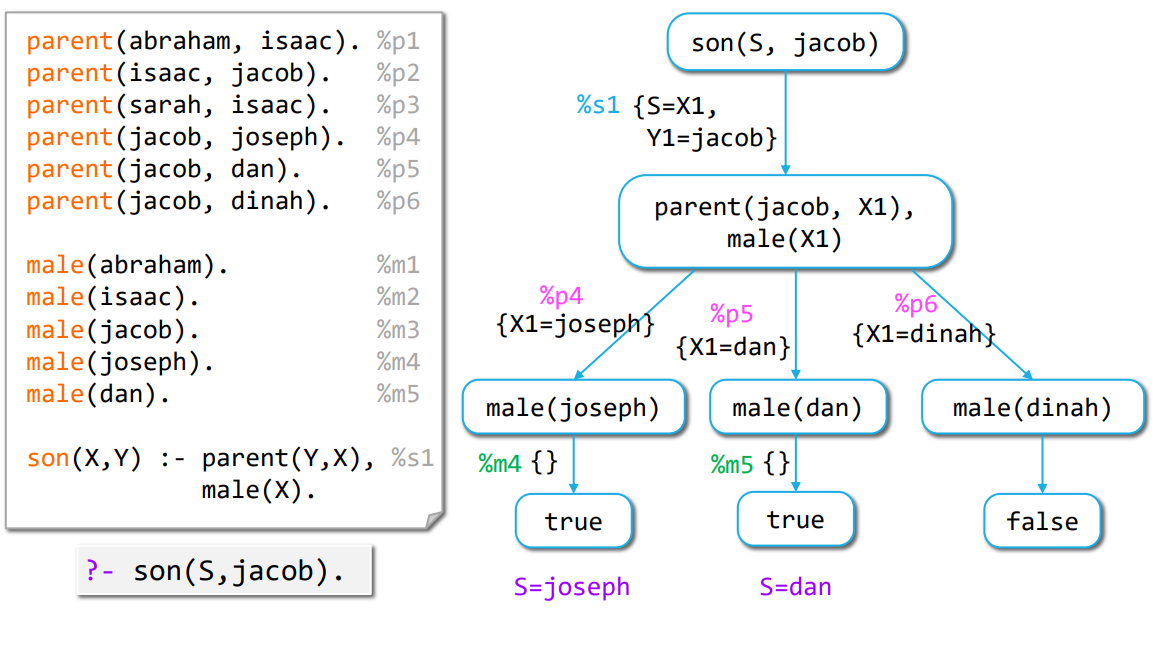
\includegraphics[width=\linewidth]{figures/proof-tree.png}
    \caption{An example of proof tree generated by the SLD resolution principle while attempting to prove the goal $son(S, \functor{jacob})$ against the depicted knowledge base. }
    \label{fig:proof-tree}
\end{figure}

\Cref{fig:proof-tree} exemplifies the proof tree generated by the recursive application of SLD inference rule to the goal $son(S, \functor{jacob})$.
%
The resolution attemps to prove the goal against a knowledge base describing Abraham's family tree, represented in the same image.
%
Each node in the tree represents a rewritten form of the original goal, whereas each arc subtends the selection of a rule from the knowledge base and a literal from the source node: the label of each edge describes their MGU.

Of course, at each step of the SLD resolution, several choices may be taken.
%
For instance, several literals may be selected, and each literal may unify with potentially many rules in the knowledge base.
%
The theorerical formulation of the SLD principle addresses such choices via \emph{non-determinism}.
%
However, whenever an actual computational agent needs to perform automated reasoning, it must leverage upon some smart strategy to explore the proof tree sequentially, and in useful time.

\paragraph{Colmerauer's Prolog}

Prolog \cite{ColmerauerR93} is the most successful expression of the LP paradigm.
%
It is at the same time a particular way of expressing logic resolution, and a very powerful technology to perform automated reasoning in practice.
%
Here we focus on the theoretical aspects of Prolog, whereas technological aspects are treated later in this thesis.

Prolog is essentially a particular way to make the exploratioon of the proof tree subtended by the SLD resolution principle \emph{sequential}.
%
In other words, Prolog makes the SLD resolution a sequential algorithm.
%
More precisely, Prolog assumes goals to be \emph{ordered} disjunctions of literals (left to right), and knowledge bases to be \emph{ordered} sets of definite clauses (top to bottom).
%
Under such assumption, it adopts the following stategy while dealing with the non-determinism of SLD resolution:
%
\begin{itemize}
    \item literals in the current goal are reduced from left to right,
    \item rules are selected from top to bottom.
\end{itemize}
%
This strategy subtends a \emph{depth-first} exploration of the proof tree.

Another relevant modelling choice in Prolog concerns the syntax for predicates and terms.
%
In fact, Prolog represents predicates and structured terms in the same way, collapsing their syntaxes and making the two notions interchangeable.
%
This simplifies the definition of meta-predicates -- i.e. predicates accepting other predicates as arguments --, as terms can be used to represent predicates.
%
Meta-predicates, in turn, make Prolog's semantics very flexible, as disjunctions, implications, negations, and many other features of FOL which are not supported by Horn clauses can be re-introduced in Prolog in this way.

\paragraph{Clark's Negation as Failure}

NaF \cite{Clark77} is the last relevant extension of SLD we discuss in this section.
%
It essentially aims at supporting negation in Horn clauses.
%
SLD resolution extended with NaF is often concisely referred to as SLDNF.

SLDNF supports negation by defining the meta-predicate $not(g)$ which is proven true if and only if the argument goal $g$ is proven unsatisfiable.
%
So, in procedural terms, the goal $not(g)$ can be read as ``attempt to prove $g$, and, if no solution exists, then $not(g)$ is true, false otherwise''.

Notably, NaF subtends a \emph{closed} world assumption, where everthing that is not know -- nor deducible from what is known -- is false.

\section{Sub-symbolic Reasoning}

Inference in ML = application of learned models to novel data.

A number of recent proposals are however pushing relevant aspects of logic and inference into the sub-symbolic realm.
%
We classify such efforts according to 3 categories, namely:
%
\begin{itemize}
    \item approaches where symbolic information is used to structure or constrain the behaviour of a sub-symbolic system
    \item approaches where symbolic information is sub-symbolically processed
\end{itemize}

\subsection{Neuro-Symbolic Integration}



\subsection{Knowledge Graph Embedding}

\chapter{Explaining AI via Symbolic Knowledge}

Despite the open philosophical issues, it is undeniable that AI and ML are nowadays becoming more and more intertwined with a growing number of aspects of people's every day life \cite{helbing2019, elliott2019}. 
%
In fact, more and more decisions are delegated by humans to software agents whose intelligent behaviour is not the result of some skilled developer endowing it with some clever code, but rather the consequence the agents' capability of learning, planning, or inferring what to do from data.

In spite of the large adoption, intelligent machines whose behaviour is the result of automatic synthesis / learning procedures are difficult to trust for most people---in particular when they are not expert in the field.
%
This is especially true for agents leveraging on machine or deep learning based techniques, often producing models whose internal behaviour is opaque and hard to explain for their developers too.

There, agents often tend to accumulate their knowledge into \emph{black-box} predictive models which are trained through ML or DL.
%
Broadly speaking, the ``black-box'' expression is used to refer to models where knowledge is not explicitly represented -- such as in NN, support vector machines (SVM), or random forests --, and it is therefore difficult, for humans, to understand what a black-box actually knows, or what leads to a particular decision.

Such difficulty in understanding black-boxes content and functioning is what prevents people from fully trusting -- and thus accepting -- them.
%
In several contexts, such as the medical or financial ones, it is not sufficient for intelligent agents to output bare decisions, since, for instance, ethical and legal issues may arise. 
%
An \emph{explanation} for each decision is therefore often desirable, preferable, or even required.  
%
Furthermore, it may happen for instance that black-boxes \emph{silently} learn something wrong (e.g., Google image recognition software that classified black people as gorillas \cite{fourcade2017, crawford2016artificial}), or something right, but in a biased way (like  the ``background bias'' problem, causing for instance husky images to be recognised only because of their snowy background \cite{RibeiroSG16}).

To tackle such trust issues, the \emph{eXplainable Artificial Intelligence} (XAI) research field has recently emerged, and a comprehensive research road map has been proposed by DARPA \cite{darpa2016-xai}, targeting the themes of explainability and interpretability in AI -- and in particular ML -- as a challenge of paramount importance in a world where AI is becoming more and more pervasively adopted.
%
There, DARPA reviews the main approaches to make AI either more interpretable or \emph{a posteriori} explainable, it categorises the many currently available techniques aimed at building meaningful interpretations or explanations for black-box models, it summarises the open problems and challenges, and it provides a reference framework for the researchers interested in the field.

Broadly speaking, research efforts in the field of XAI are focused on achieving key properties in AI, such as \emph{interpretability}, \emph{transparency}, \emph{explainability}, \emph{accountability}, and \emph{trustworthiness}.
%
Unfortunately, such goals are still far from being reached.
%
For instance, as pointed out in \cite{Lipton18}, the aforementioned properties are still lacking a formal and agreed-upon definition.
%
Some authors \cite{Rudin2019} propose to strengthen the adoption of most \emph{interpretable} (i.e. algorithmically transparent) predictive models -- such as generalised linear models or decision trees --, while others seek new ways to produce \emph{post-hoc} explanations capable of tackling even most opaque predictors, such as NN.
%
However, as demonstrated by the comprehensive survey produced by Guidotti et al. \cite{GuidottiMRTGP19}, most works only target classification problems, and they rarely take wider properties -- such as accountability and trustworthiness -- into account.

\sidenote{Spostare il capoverso sotto in un posto più opportuno}
Several works, among the various springs of AI, proposed to extract symbolic knowledge from sub-symbolic models.
%
As witnessed by a number of surveys \cite{GuidottiMRTGP19, GarcezBRFHIKLMS15, AndrewsDT95, GarcezBG01} and works on the topic \cite{BolognaH18, BolognaH16, FrosstH17, JohanssonN09, KrishnanSB1999, HruschkaE2006, ZhouZYS1983, CravenS95, AugastaK12, SatoT2002, KahramanliA09a} -- some of which are from the 80s or the 90s -- the potential of symbolic knowledge \emph{extraction} is well understood, despite not being subject to hype.
%
Unfortunately, a comprehensive and general framework tackling such problem in a general way is still missing.

\note{Armonizzare quanto segue con ciò che precede}

Since the adoption of interpretable predictors usually comes at cost of a lower potential in terms of predictive performance, \emph{explanations} are the newly preferred way for providing understandable predictions without necessarily sacrificing accuracy.
%
The idea, and the main goal of XAI is to create intelligible and understandable explanations for uninterpretable predictors \emph{without} replacing or modifying them.
%
Thus explanations are built through a number of heterogeneous techniques, broadly referred to as \emph{explanators} \cite{GuidottiMRTGP19}---just to cite some, \emph{decision rules} \cite{Augasta2012}, \emph{feature importance} \cite{tolomei2017interpretable}, saliency masks \cite{FongV17}, sensitivity analysis \cite{SundararajanTY17}, etc.

The state of the art for explainability currently recognises two main sorts of explanators, namely, either local or global. 
%
While \emph{local} explanators attempt to provide an explanation for each particular prediction of a given predictor $p$, the \emph{global} ones attempt to provide an explanation for the predictor $p$ as a whole.
%
In other words, local explanators provide an answer to the question ``why does $p$ predict $\mathbf{y}$ for the input $\mathbf{x}$?'' -- such as the LIME technique presented in \cite{RibeiroSG16} --, whereas global explanators provide an answer to the question ``how does $p$ build its predictions?''---such as decision rules.

In spite of the many approaches proposed to explain black boxes, some important scientific questions still remain unanswered. 
%
One of the most important open problems is that, until now, there is no agreement on what an explanation is. 
%
Indeed, some approaches adopt as explanation a set of rules, others a decision tree, others rely on visualisation techniques \cite{GuidottiMRTGP19}. 
%
Moreover, recent works highlight the importance for an explanation to guarantee some properties, e.g., soundness, completeness, and compactness \cite{GuidottiMRTGP19}. 

% \note{Probabilmente si può tagliare da qui in poi}

% This is why our proposal aims at integrating sub-symbolic approaches with symbolic ones.
% %
% To this end, DT can be exploited as an effective bridge between the symbolic and sub-symbolic realms.
% %
% In fact, DT can be easily \emph{(i)} built from an existing sub-symbolic predictor, and \emph{(ii)} translated into symbolic knowledge -- as it is shown in the reminder of this paper -- thanks to their rule-based nature.

% Decision trees are an interpretable family of predictors that have been proposed as a \emph{global} means for explaining other, less interpretable, sorts of black-box predictors \cite{TrattnerPR2019,BastaniKB17}---such as neural networks \cite{CravenS95}.
% %
% The main idea behind such an approach is to build a DT approximating the behaviour of a given predictor, possibly, by only considering its inputs and its outputs.
% %
% Such approximation essentially trades off predictive performance with interpretability.
% %
% In fact, the structure of such a DT would then be used to provide useful insights concerning the original predictor inner functioning. 

% Describing the particular means for extracting DT from black-boxes is outside the scope of this paper.
% %
% Given the vast literature on the topic -- e.g., consider reading \cite{GuidottiMRTGP19,AndrewsDT95} for an overview or \cite{CravenS95,JohanssonN09,FrosstH17} for a practical examples -- we simply assume an extracted DT is available and it has an high \emph{fidelity}---meaning that the loss in terms of predictive performance is low, w.r.t. the original black-box.
% %
% In fact, whereas there exist several works focussing on how to synthesise DT out of black-box predictors, no attention is paid to merging them with symbolic approaches, which can play a key role in enhancing the interpretability and explainability of the system.
% %
% In this paper we focus on such a matter.

% We believe that a logical representation of DT may be interesting and enabling for further research directions.
% %
% For instance, as far as explainability is concerned, we show how logic-translated DT can be used to both navigate the knowledge stored within the corresponding predictors -- thus acting as \emph{global} explanators --, and produce \emph{narrative} explanations for their predictions---thus acting as \emph{local} explanators. 
% %
% Note that the restriction on the DT representation makes it easy to map DT onto logical clauses, since DT are finite and with a limited expressivity (if / else conditions).

%===============================================================================
\section{XAI Background}\label{sec:background}
%===============================================================================

Most intelligent systems (IS) today leverage on \emph{numerical} predictive models which are trained from data through ML.
%
The reason for such a wide adoption is easy to understand.
%
We live in an era where the availability of data is unprecedented, and ML algorithms make it possible to semi-automatically detect useful statistical information hidden into such data.
%
Information, in turn, supports decision-making, monitoring, planning, and forecasting in virtually any human activity where data is available.

However, ML is not the silver bullet.
%
Despite the increased predictive power, ML comes with some well-known drawbacks which make it perform poorly in some use cases.
%
One blatant example is algorithmic \emph{opacity}---that is, essentially, the difficulty of human mind in \emph{understanding} how ML-based IS function or compute their outputs.
%
Such difficulty is a serious issue in all those contexts where human beings are liable for their decision or must provide some sort of \emph{explanation} for it---even if the decision has been supported by some IS.
%
For instance, think about a doctor willing to motivate a serious, computer-aided diagnosis, or, a bank employee in need of explaining to a customer why his/her profile is inadequate for a loan.
%
In all contexts, ML is at the same time an enabling -- as it aids the decision process by automating it -- and a limiting factor---as opacity prevents human awareness of \emph{how} the decision process works.

Opacity is why ML predictors are also referred to as \emph{black boxes} into the literature.
%
The ``black box'' expression refers to models where knowledge is not explicitly represented \cite{Lipton18}. 
%
The lack of some explicit, symbolic representation of knowledge is what makes it hard for humans to \emph{understand} the functioning of black boxes, and why they led to suggest or undertake a given decision.
%
Obviously, troubles in understanding black-box content and functioning prevents people from fully trusting -- therefore accepting -- them. 
%
To make the picture even more complex, current regulations such as the GDPR \cite{gdpr-voigt2017} are starting to recognise the citizens' \emph{right to explanation} \cite{explanation-aimag38}---which implicitly requires IS to eventually become \emph{understandable}.
%
In fact, understanding IS is essential to guarantee algorithmic fairness, to identify potential bias/problems in the training data, and to ensure that IS perform as designed and expected. 

%%%%
\begin{figure}
    \centering
    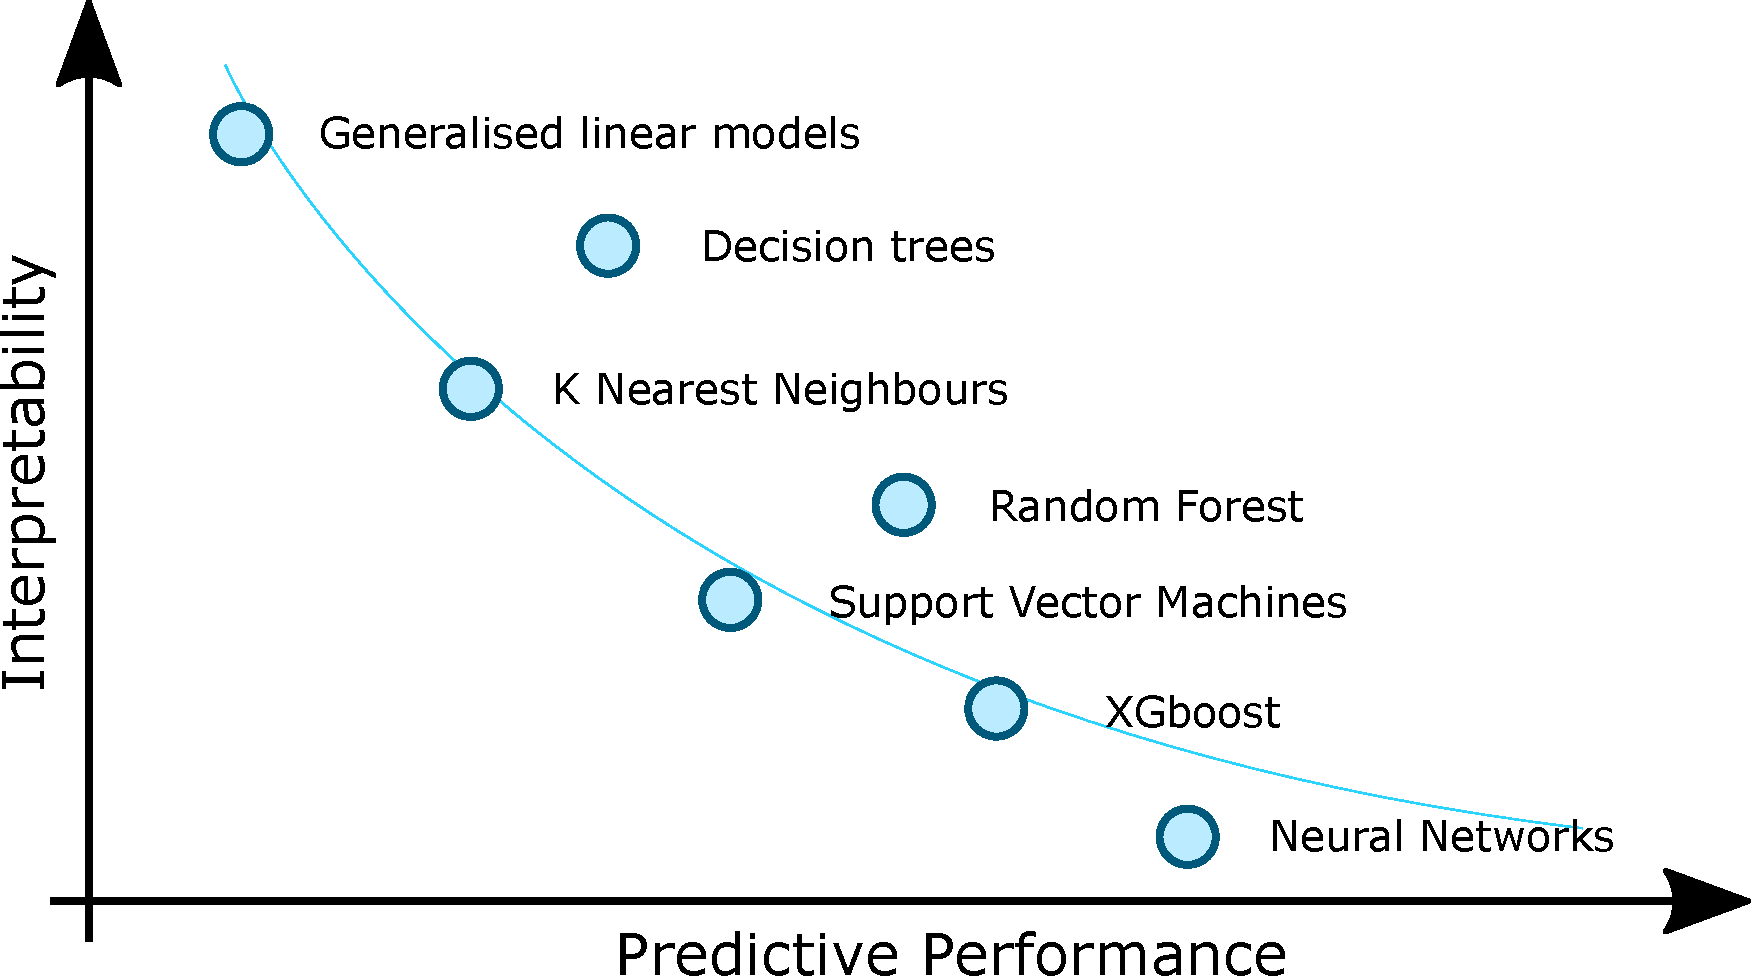
\includegraphics[width=.5\linewidth]{figures/interpretability-performance-tradeoff}
    \caption[Interpretability/performance trade-off]{Interpretability/performance trade-off for some common sorts of black-box predictors}
    \label{fig:tradeoff}
\end{figure}
%%%%

Unfortunately, the notion of understandability is neither standardised nor systematically assessed, yet.
%
At the same time, there is no consensus on what exactly providing an \emph{explanation} should mean when decisions are supported by a black box.
%
However, several authors agree that not all black boxes are equally \emph{interpretable}---meaning that some black boxes are easier to understand than others for our mind.
%
For example, \Cref{fig:tradeoff} is a common way to illustrate the differences in black-box interpretability.

Even though informal -- as pointed on in \cite{Rudin2019}, given the lack of way to measure ``interpretability'' -- \Cref{fig:tradeoff} effectively express why more research is need on understandability.
%
In fact, the image essentially states how the better performing black boxes are also the less interpretable ones.
%
This is a problem in practice since only rarely predictive performances can be sacrificed in favour of an higher degree of interpretability.

To tackle such issues, the \emph{eXplainable AI} (XAI henceforth) research field has recently emerged.
%
Among the many authors and organisations involved in the topic, DARPA has proposed a comprehensive research road map \cite{darpa2016-xai} which reviews the main approaches to make black boxes more understandable.
%
There, DARPA categorises the many currently available techniques aimed at building meaningful interpretations or explanations for black-box models, it summarises the open problems and challenges, and it provides a successful reference framework for the researchers interested in the field.
%
Unfortunately, in spite of the great effort in defining terms, objects, and methods for the research line, a clear definition of fundamental notions such as \emph{interpretation} and \emph{explanation} is still missing.

%-------------------------------------------------------------------------------
\subsection{Related works}\label{ssec:related}
%-------------------------------------------------------------------------------

Notions such as explanation, interpretation, transparency, etc, are mentioned, introduced, or informally defined in several works.
%
However, a coherent framework has not emerged yet.

In this subsection we recall some of the main contributions from the literature where the concepts of explanation and interpretation -- or any variant of theirs -- are discussed.
%
Our goal here is to highlight the current lack of consensus on the meaning of such terms, for which we propose a possible, unambiguous alternative in the next sections.

Similarly to what we do here, Lipton \cite{Lipton18} starts his discussion by recognising how most definition of ML interpretability are often inconsistent and underspecified.
%
In his clarification effort, Lipton essentially maps interpretability on the notion of \emph{transparency}, and explanation on the notion of \emph{post-hoc} interpretation.
%
Then, he enumerates and describes the several possible variants of transparency, that are 
%
\begin{enumerate*}[label=\emph{(\roman{*})}]
    \item simulatability -- i.e., the \emph{practical} possibility, for a human being, to ``contemplate the entire model at once'' and simulate its functioning on some data  -- which characterises, for instance, generalised linear models;
    
    \item decomposability -- i.e., the possibility, for the model to be decomposed in elementary parts whose functioning is intuitively understandable for humans and helpful in understanding the whole model -- which characterises, for instance, decision trees; and
    
    \item algorithmic transparency -- i.e., the possibility, for a human being, to intuitively understand how a given learning algorithm, or the predictors it produces, operate -- which characterises, for instance, k-nearest-neighbours techniques.
\end{enumerate*}
%
Similarly, \emph{post-hoc} interpretability is defined as an approach where some information is extracted from a black box in order to ease its understanding.
%
Such information have not necessarily to expose the internal functioning of the black box.
%
As stated in the paper: ``examples of post-hoc interpretations include the verbal explanations produced by people or the saliency maps used to analyze deep neural networks''.

Conversely, Besold et al. \cite{BesoldU2018} discuss the notion of explanation at a fundamental level.
%
There, the authors provide a nice philosophical overview on such topic, concluding that ``explanation is an epistemological activity and explanations are an epistemological accomplishment---they satisfy a sort of epistemic longing, a desire to know something more than we currently know. Not only do they satisfy this desire to know, they also provide the explanation-seeker a direction of action that they did not previously have''.
%
Then they discuss the topic of explanation in AI from an historical perspective.
%
In particular, when focussing on ML, they introduce the following classification of IS systems:
%
\begin{enumerate*}[label=\emph{(\roman{*})}]
    \item opaque systems -- i.e., black boxes acting as oracles where the logic behind predictions is not observable or understandable --,
    
    \item interpretable systems -- i.e., white boxes whose functioning is understandable to humans, also thanks to expertise, resources, or tools --, and
    
    \item comprehensible systems---i.e., ``systems which emit \emph{symbols} along with their outputs, allowing the user to relate properties of the input to the output''.
\end{enumerate*}
%
According to this classification, while interpretable systems can be inspected to be understood -- thus letting observer draw their explanations by themselves--, comprehensible systems must explicitly provide a symbolic explanation of their functioning.
%
The focus there is thus on \emph{who} produces explanations, rather than \emph{how}.

In \cite{DoshiVelezK2017}, interpretability of ML systems is defined as ``the ability to explain or to present in understandable terms to a human''.
%
Interpretations and explanations are therefore collapsed in this work, as confirmed by the authors using the two terms interchangeably.
%
The reminder of that paper focuses 
\begin{enumerate*}[label=\emph{(\roman{*})}]
    \item on identifying under which circumstances interpretability is needed in ML, and
    \item how to assess the quality of some explanation.
\end{enumerate*}

The survey by Guidotti et al. \cite{GuidottiMRTGP19} is a nice entry point to explainable ML.
%
It consists of an exhaustive and recent survey overviewing the main notions, goals, problems, and (sub-)categories in this field and it encompasses a taxonomy of existing approaches for ``opening the black box''---which may vary a lot depending on the sort of data and the family of predictors at hand.
%
There, the authors define the verb to interpret as the act of ``providing some meaning of explaining and presenting in understandable terms some concepts'', borrowing such a definition from the Merriam-Webster\footnote{\url{https://www.merriam-webster.com/dictionary/interpret}} dictionary.
%
Consequently, they define interpretability as ``the ability to explain or to provide the meaning in understandable terms to a human''---a definition they again borrow from \cite{DoshiVelezK2017}.
%
So, in this case as well the notions of \emph{interpretation} and \emph{explanations} are collapsed.

In \cite{Rudin2019}, Rudin does not explicitly provide a definition for explainability or interpretability, and she refers about interpretable or explainable ML almost interchangeably.
%
However, she states some interesting properties about \emph{interpretability}, which influenced our work.
%
In particular, she acknowledges that ``interpretability is a domain-specific notion''.
%
Furthermore, she links interpretability of information with its complexity -- and, in particular, its \emph{sparsity} --, as the amount of cognitive entities the human mind can at one is very limited ($\sim 7 \pm 2$ according to \cite{numberseven-psyrev63}). 
%
As far as explainability is concerned, apparently, Rudin adopts a \emph{post-hoc} perspective similar to the one in \cite{Lipton18}, as she writes ``an explanation is a separate model that is supposed to replicate most of the behaviour of a black box''.
%
In the reminder of the paper, the author argues how the path towards interpretable ML steps through a wider adoption of inherently interpretable predictors -- such as generalised linear models or decision trees -- instead of the relying on \emph{post-hoc} explanations which do not reveal what is inside black boxes---thus preventing their full understanding.

Finally, the recent article by Rosenfeld et al. \cite{RosenfeldR2019} is similar in its intents to our current work.
%
There, the authors attempt to formally define what explanation and interpretation respectively are in the case of ML-based classification. 
%
However, their work differs from ours in several ways.
%
In particular, they define interpretation and explanation differently from what we do.
%
In fact, according to the authors, ``interpretation'' is a function mapping data, data schemes, and predictors to some representation of the predictors internal logic, whereas ``explanation'' is defined as ``the human-centric objective for the user to understand'' a predictor using the aforementioned interpretation function.
%
Other notions are formally defined into the paper, such as for instance, 
%
\begin{inlinelist}
    \item explicitness, 
    \item fairness, 
    \item faithfullness,
    \item justification, and
    \item transparency.
\end{inlinelist}
%
Such concepts are formally defined in terms of the aforementioned interpretation and explanation functions.
%
The reminder of the paper then re-interprets the field of XAI in terms of all the notions mentioned so far. 

\section{Explanation vs. Interpretation}\label{sec:basics}

This section introduces the preliminary notions, intuitions, and notations we leverage upon in \cref{ssec:framework} and subsequent sections, in order to formalise our abstract framework for agent-based explanations.
%
We start by providing an intuition for the notion of \emph{interpretation}, and, consequently, for the \emph{act} of interpreting something.
%
Accordingly, we provide an intuition for the property of ``being interpretable'' as well, stressing its comparative nature.
%
Analogously to what we did with \emph{interpretation}, we then provide intuitions for terms such as \emph{explanation} and its derivatives.

%---
\paragraph{About interpretation}
%---

Taking inspiration from the field of Logics, we define the \emph{act} of ``interpreting'' some object $X$ as the activity performed by an agent $A$ -- either human or software -- assigning a \emph{subjective} meaning to $X$.
%
Such meaning is what we call \emph{interpretation}.
%
Roughly speaking, an object $X$ is said to be  \emph{interpretable} for an agent $A$ if it is \emph{easy} for $A$ to draw an interpretation for $X$---where ``easy'' means $A$ requires a low \emph{computational} (or \emph{cognitive}) effort to understand $X$.
%
For instance, consider the case of road signs, which contain symbols instead of scripts to be easily, quickly, and intuitively interpretable.

We model such intuition through a function $I_A(X) \mapsto [0, 1]$ providing a \emph{degree of interpretability} -- or simply interpretability, for short -- for $X$, in the eyes of $A$.
%
The value $I_A(X)$ is not required to be directly observable or measurable in practice, since agents' mind may be inaccessible in most cases.
%
This is far from being an issue, since we are not actually interested in the absolute value of $I_A(X)$, for some object $X$, but rather we are interested in being able to order different objects w.r.t.\ their subjective interpretability.
%
For instance, we write $I_A(X) > I_A(Y)$, for two objects $X$ and $Y$, meaning that the former is more interpretable than the latter, according to $A$.
%
For example, consider the case of a neural network and a decision tree, both trained on the same examples to solve the same problem with similar predictive performances.
%
Both objects may be represented as graphs.
%
However, it is likely for a human observer to see the decision tree as more interpretable---as their nodes bring semantically meaningful, high-level information.

Summarising, we stress the subjective nature of interpretations, as agents assign them to objects according to their State of Mind (SoM) \cite{PremackW1978} and background knowledge, and they need not be formally defined any further.

%%%%
\begin{figure}
    \centering
    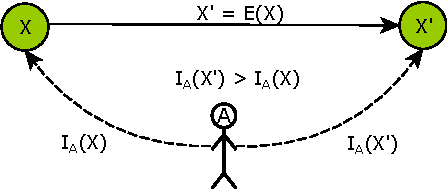
\includegraphics[width=.5\linewidth]{figures/framework.pdf}
    \caption{Explanation vs. Interpretation: a simple framework}
    \label{fig:framework}
\end{figure}
%%%%

%---
\paragraph{About explanation}
%---
We define ``explaining'' as the activity of producing a more interpretable object $X'$ out of a less interpretable one, namely $X$, performed by agent $A$.
%
More formally, we define \emph{explanation} as a function $E(X) \mapsto X'$ mapping objects into other objects, possibly, in such a way that $I_A(X') > I_A(X)$, for some agent $A$.
%
The simple framework described so far is summarised in \cref{fig:framework}.

Notice that human beings tend to collapse into the concept of ``explanation'' the whole sequence of steps actually involving both explaining and interpreting, according to our framework.
%
This happens because, if the explained object $X'$ is as interpretable for the listening agent $B$ as it is for the explaining agent $A$, then both $A$ and $B$ are likely to be satisfied with $X'$.
%
Conversely, it may also happen the explanation $E$ adopted by $A$ produces an object $X'$, which is more interpretable than $X$ for $A$ but not for $B$.
%
Similarly to how two persons would handle such an unpleasant situation, we envision that interaction and communication may be adopted to break such \emph{impasses} in multi-agent systems.

In the following sections, we develop such an idea, describing how our simple framework could be extended to support ML-based intelligent systems.

%-------------------------------------------------------------------------------
\subsection{A conceptual framework for XAI}\label{ssec:framework}
%-------------------------------------------------------------------------------

In AI several tasks can be reduced to a functional model $M: X \rightarrow Y$ mapping some input data $X \subseteq \mathcal{X}$ from an input domain $\mathcal{X}$ into some output data $Y \subseteq \mathcal{Y}$ from an output domain $\mathcal{Y}$.

In the following, we denote as $\mathcal{M}$  the set of all \emph{analogous} models $M': X \rightarrow \mathcal{Y}$, which attempts to solve the same problem on the same input data---usually, in (possibly slightly) different ways.
%
For instance, according to this definition, a decision tree and a neural network, both trained on the same data-set to solve the same classification problem with similar accuracies, are analogous---even if they belong to different families of predictors.

At a very high abstraction level, many tasks in AI may be devoted to compute, for instance:
%
\begin{itemize}
    \item the best $M^* \in \mathcal{M}$, given $X \subseteq \mathcal{X}$ and $Y \subseteq \mathcal{Y}$ (e.g. supervised ML),
    \item the best $M^*$ and $Y$, given $X$ (e.g.\ unsupervised ML),
    \item the best $Y^*$, given $X$ and $M$ (e.g.\ informed/uninformed search),
    \item the best $X^*$, given $Y$ and $M$ (e.g.\  abduction, most likely explanation), etc 
\end{itemize}
%
according to some goodness criterion which is specific for the task at hand.

In the reminder of this section, we discuss how explanation may be defined as a function searching or building a -- possibly more interpretable -- model w.r.t.\ the one to be explained.
%
For this process to even make sense, of course, we require the resulting model to be not only analogous to the original but also similar in the way it behaves on the same data.
%
We formalise such a concept through the notion of \emph{fidelity}.

Let $M, M' \in \mathcal{M}$ be two analogous models.
%
We then say $M$ has a \emph{locally} good \emph{fidelity} w.r.t.\ $M'$ and $Z$ if and only if $\Delta f(M(Z), M'(Z)) < \delta$ for some arbitrarily small threshold $\delta \geq 0$ and for some subset of the input data $Z \subset X$.
%
There, $\Delta f : 2^\mathcal{Y} \times 2^\mathcal{Y} \rightarrow \mathbb{R}_{\geq 0}$ is a function measuring the performance \emph{difference} among two analogous models.

%%%%
\begin{figure}
    \centering
    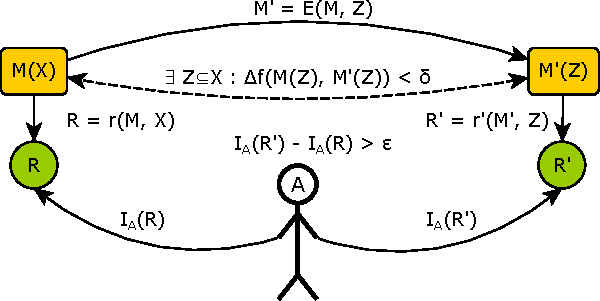
\includegraphics[width=.5\linewidth]{figures/local.pdf}
    \caption{Local explanation and interpretation of a model}
    \label{fig:local}
\end{figure}
%%%%

%---
\paragraph{Local interpretations}
%---

When an observer agent $A$ is \emph{interpreting} a model $M$ behaviour w.r.t.\ some input data $Z \subseteq X$, it is actually trying to assign a subjective interpretability value $I_A(R)$ to some representation $R = r(M, Z)$ of choice, aimed at highlighting the behaviour of $M$ w.r.t.\ the data in $Z$.
%
There, $r : \mathcal{M} \times 2^\mathcal{X} \rightarrow \mathcal{R}$ is \emph{representation means}, i.e., a function mapping models into \emph{local} representations w.r.t.\ a particular subset of the input domain, whereas $\mathcal{R}$ is the set of model representations.
%
For instance, in the case $M$ is a classifier, $R$ may be a graphical representation of (a portion of) the decision boundary/surface for a couple of input features.

There may be more or less interpretable \emph{representations} of a particular model for the same observer $A$.
%
Furthermore, representations may be either global or local as well, depending on whether they represent the behaviour of the model for the whole input space, or for just a portion of it.
%
For example, consider the case of a plot showing the decision boundary of a neural network classifier.
%
This representation is likely far more interpretable to the human observer than a graph representation showing the network structure, as it synthesise the global behaviour of the network concisely and intuitively.
%
Similarly, saliency maps are an interpretable way to \emph{locally} represent the behaviour of a network w.r.t. some particular input image.
%
So, a way for easing interpretation for a given model behaviour w.r.t.\ a particular sort of inputs is about looking for the right representation in the eyes of the observer.

%---
\paragraph{Local explanations}    
%---

Conversely, when an observer $A$ is \emph{explaining} a model $M$ w.r.t.\ some input data $Z \subseteq X$, it is actually trying to produce a model $M' = E(M, Z)$ through some function $E: \mathcal{M} \times 2^\mathcal{X} \rightarrow \mathcal{M}$.
%
In this case, we say $M'$ is a \emph{local explanation} for $M$ w.r.t.\ to $Z$.
%
We also say that $M'$ is produced through the explanation strategy $E$.

Furthermore, we define an explanation $M'$ as \emph{admissible} if it has a valid fidelity w.r.t.\ the original model $M$ and the data in $Z$---where $Z$ is the same subset of the input data used by the explanation strategy.
%
More precisely, we say $M'$ is $\delta$-admissible in $Z$ w.r.t.\ $M$ if $\Delta f(M(Z), M'(Z)) < \delta$.

Finally, we define an explanation $M'$ as \emph{clear} for $A$, in $Z$, and w.r.t.\ the original model $M$, if there exists some representation $R' = r(M', Z)$ which is more interpretable than the original model representation $R$.
%
More precisely, we say $M'$ is $\varepsilon$-clear for $A$, in $Z$, and w.r.t $M$ if $I_A(R') - I_A(R) > \varepsilon$ for some arbitrarily big threshold $\varepsilon > 0$.

Several \emph{explanations} may actually be produced for the same model $M$.
%
For each explanation, there may be again more or less interpretable \emph{representations}.
%
Of course, explanations are useful if they ease the seek for more interpretable representations.
%
Thus, providing an explanation for a given model behaviour w.r.t.\ a particular class of inputs is about creating \emph{ad-hoc} metaphors aimed at easing the observer's understanding.

%%%%
\begin{figure}
    \centering
    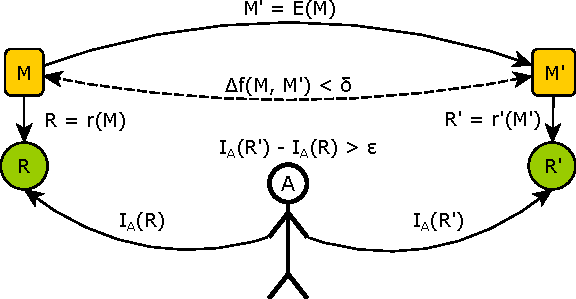
\includegraphics[width=.5\linewidth]{figures/global.pdf}
    \caption{Global explanation and interpretation of a model}
    \label{fig:global}
\end{figure}
%%%%

%---
\paragraph{Global / local explanations}
%---

The theoretical framework described so far -- which is graphically synthesised in \cref{fig:local} -- is aimed at modelling \emph{local} interpretations and explanations, that are, the two means an explanator agent may exploit in order to make AI tasks' \emph{outcomes} more understandable in the eyes of some explanee. 

Conversely, when the goal is not to understand some model outcome, but the model itself, from a \emph{global} perspective -- or, equivalently, when the goal is to understand the model outcome w.r.t the whole set of input data $X$ --, the theoretical framework described so far is simplified as shown in \cref{fig:global}, where the dependency on the input data is omitted from functions $E$, $\Delta f$, and $r$.
%
This is possible because we consider the global case as a particular case of the local one, where $Z \equiv X$.

Finally, we remark that the case where a model $M$ is to be understood on a single input-output pair, say $x$ and $y = M(x)$, is simply captured by the aforementioned local model, through the constraint $Z = \{ x \}$ and $M(Z) = \{ y \}$.

%-------------------------------------------------------------------------------
\subsection{Discussion}
%-------------------------------------------------------------------------------

Our framework is deliberately abstract in order to capture a number of features we believe to be essential in XAI.
%
First of all, our framework acknowledges -- and properly captures -- the orthogonality of interpretability w.r.t.\ explainability. 
%
This is quite new, indeed, considering that most authors tend to use the two concepts as if they were equivalent or interchangeable.

Furthermore, our framework explicitly recognises the \emph{subjective} nature of interpretation, as well as the subtly \emph{objective} nature of explanation.
%
Indeed, interpretation is a subjective activity directly related to agents' perception and SoM, whereas explanation is an epistemic, computational action which aims at producing a high-fidelity model.
%
The last step is objective in the sense that it does not depend on the agent's perceptions and SoM, thus being reproducible in principle.
%
Of course, the \emph{effectivess} of an explanation is again a subjective aspect.
%
Indeed, a clear explanation (for some agent) is a more interpretable variant of some given model--- thus, the subjective activity of interpretation is again implicitly involved.

The proposed framework also captures the importance of representations.
%
This is yet another degree of freedom that agents may exploit in their seek for a wider understandability of a given model.
%
While other frameworks consider interpretability as an intrinsic property of AI models, we stress the fact that a given model may be represented in several ways, and each representation may be interpreted differently by different agents.
%
As further discussed in the remainder of this paper, this is far from being an issue.
%
This subjectivity is deliberate, and it is the starting point of some interesting discussions.

Finally, our framework acknowledges the global/local duality of both explanation and interpretation, thus enabling AI models to be understood either general or with respect to a particular input/output pair.

%-------------------------------------------------------------------------------
\subsection{Practical remarks}
%-------------------------------------------------------------------------------

The ultimate goal of our framework is to provide a general, flexible, yet minimal framework describing the many aspects concerning AI understandability in the eyes of a \emph{single} agent.
%
We here illustrate several practical issues affecting our framework in practice, and further constraining it.

According to our conceptual framework, a \emph{rational} agent seeking to understand some model $M$ (or make it understandable) may either choose to elaborate on the \emph{interpretation axis} -- thus looking for a (better) representation $R$ of $M$ -- or it can elaborate on the \emph{explainability axis}---thus producing a novel, high fidelity model $M'$, coming with a representation $R'$ which is more interpretable than the original one (i.e., $R$).

Notice that, in practice, the nature of the model constrains the set of admissible representations.
%
This means that a rational agent is likely to exploit both the explanation and interpretation axes in the general case---because novel representations may become available through an explanation.
%
we argue and assume that each family of AI models comes with just a few \emph{natural} representations.
%
Because of this practical remark, we expect that, in real-world scenarios, an agent seeking for understandability is likely to ``work'' on both the interpretation and the explanation axes.

For instance, consider decision trees, which come with a natural representation as a tree of subsequent choices leading to a decision.
%
Conversely, neural networks can either be represented as graphs or as algebraic combinations of tensors.
%
In any case, neural network models are commonly considered less interpretable than other models.
%
In such situation, a rational agent willing to make a neural network more understandable may choose to combine decision trees extraction (explanation) -- possibly focusing on methods from the literature \cite{AndrewsDT95,xailp-woa2019} -- to produce a decision tree whose tree-like structure (representation) could be presented to the human observer to ease his/her interpretation.
%
The decision-tree like representation is not ordinarily available for neural networks, but it may become available provided that an explanation step is performed.

Another interesting trait of our framework concerns the semantics of clear explanations.
%
The current definition requires explanation strategies to consume a model $M$ with a given representation $R$ and to produce a high-fidelity model $M'$ for which a representation $R'$ exists, which is more interpretable than $R$.
%
Several semantics may fit this definition.
%
This is deliberate, since different semantics may come with different computational requirements, properties, and guarantees.
%
For instance, one agent may be interested in finding the \emph{best} explanation---that is, the one for which \emph{each} representation is more interpretable than the most interpretable representation of the original model.
%
Similarly, in some cases, it may be sufficient -- other than more feasible -- to find an \emph{admissible} explanation---that is, a high-fidelity model for which \emph{some} representation exists that is more interpretable than \emph{some} representation of the original model. 
%
However, the inspection of the possible semantics and their properties falls outside the scope of this paper and is going to be considered as a future research direction.

\subsection{Assessment of the Framework}\label{sec:validation}

The abstraction level of the presented framework has also been conceived in order to capture most of the current state of the art.
%
Along this line, this section aims at validating the fitting of the existing contributions w.r.t.\ the framework presented in section \cref{ssec:framework}: if our framework is expressive enough, it should allow most (if not all) existing approaches to be uniformly framed, to be easily understood and compared.
%
To this end, we leverage on the work by Guidotti et al.\ \cite{GuidottiMRTGP19}, where the authors perform a detailed and extensive survey on the state-of-the-art methods for XAI, by categorising the surveyed methods according to an elegant taxonomy.
%
Thus, hereafter, we adopt their taxonomy as a reference for assessing our framework.

The taxonomy proposed by Guidotti et al.\ essentially discriminates among two main categories of XAI methods.
%
These are the ``transparent box design'' and the ``black-box explanation'' categories. 
%
While the former category is not further decomposed, the latter comes with three more sub-categories, such as ``model explanation'', the ``outcome explanation'', and the ``model inspection''.
%
Notice that, despite the authors' definition of ``explanation'' does not precisely match the one proposed in this paper, we maintained the original categorisation.

The remainder of this section navigates such a taxonomy accordingly, by describing how each (sub-)category -- along with the methods therein located -- fits our abstract framework.

%-------------------------------------------------------------------------------
\subsubsection{Model explanation}
%-------------------------------------------------------------------------------

The mapping of the methods classified as part of the ``model explanation'' sub-category into our framework is seamless.
%
Hence, it can be defined as follows:
%
\begin{itemize}
    \item[] Let $M$ be a sub-symbolic classifier whose internal functioning representation $R$ is poorly interpretable in the eyes of some explanee $A$, and let $E(\cdot)$ be some \emph{global} explanation strategy.
    %
    Then, the model explanation problem consists of computing some \emph{global} explanation $M' = E(M)$ which is $\delta$-admissible and $\varepsilon$-clear w.r.t.\ to $A$, for some $\delta, \varepsilon > 0$. 
\end{itemize}
%
For instance, according to Guidotti et al., possible sub-symbolic classifiers are neural (possibly deep) networks, support vector machines, and random forests.
%
Conversely, explanation strategies may consist of algorithms aimed at 
%
\begin{enumerate*}[label=\emph{(\roman{*})}]
    \item extracting decision trees/rules out of sub-symbolic predictors and the data they have been trained upon, 
    \item compute feature importance vectors,
    \item detecting saliency masks,
    \item detecting partial dependency plots, etc. 
\end{enumerate*}

In our framework, all the algorithms mentioned above can be described as \emph{explanation strategies}. 
%
Such mapping is plausible given their ability to compute an admissible, and possibly more explicit models out of black boxes and the data they have been trained upon.
%
However, it is worth to highlight that the clarity gain produced by such explanation strategies mostly relies on the implicit assumption that their output models come with a natural representation which is intuitively interpretable to the human mind.

%-------------------------------------------------------------------------------
\subsubsection{Outcome explanation}
%-------------------------------------------------------------------------------

Methods classified as part of the ``outcome explanation'' sub-category can be very naturally described in our framework as well.
%
In fact, it can be defined as follows:
%
\begin{itemize}
    \item[] Let $M$ be some sub-symbolic classifier whose internal functioning representation $R = r(M, Z)$ in some subset $Z \subset \mathcal{X}$ of the input domain is poorly interpretable to some explanee $A$, and let $E(\cdot, \cdot)$ be some \emph{local} explanation strategy.
    %
    Then, the outcome explanation problem consists of computing some \emph{local} explanation $M' = E(M, Z)$ which is $\delta$-admissible and $\varepsilon$-clear w.r.t.\ to $A$, for some $\delta, \varepsilon > 0$
\end{itemize}
%
Summarising, while input black boxes may still be classifiers of any sort, explanation, and explanation strategies differ from the ``model explanation'' case.
%
In particular, explanation strategies in this sub-category may rely on techniques leveraging on attention models, decision trees/rules extraction, or well-established algorithms such as LIME \cite{RibeiroSG16}, and its extensions---which are essentially aimed at estimating the contribution of every input feature of the input domain to the particular outcome of the black box to be explained.

Notice that the explanation strategies in this category are only required to be admissible and clear in the portion of the input space surrounding the input data under study.
%
Such a portion is implicitly assumed to be relatively small in most cases.
%
Furthermore, the explanation strategy is less constrained than in the global case, as it is not required to produce explanations elsewhere.

%-------------------------------------------------------------------------------
\subsubsection{Model inspection}
%-------------------------------------------------------------------------------

Methods classified as part of the ``model inspection'' sub-category can be naturally defined as follows:
%
\begin{itemize}
    \item[] Let $M$ be a sub-symbolic classifier whose available \emph{global} representation $R = r(M)$ is poorly interpretable to some explanee $A$, and let $r(\cdot), r'(\cdot)$ be two different representation means.
    %
    Then, the model inspection problem consists of computing some representation $R' = r'(M)$ such that $I_A(R') > I_A(R)$
\end{itemize}
%
Of course, solutions to the model inspection problem vary a lot depending on which specific representation means $r(\cdot)$ is exploited by the explanator, other than the nature of the data the black box is trained upon.
%
Guidotti et al.\ also provide a nice overview of the several sorts of representations means which may be useful to tackle the model inspection problem, like, for instance, sensitivity analysis, partial dependency plots, activation maximization images, tree visualisation, etc.

It is worth pointing out the capability of our framework to reveal the actual nature of the inspection problem.
%
Indeed, it clearly shows how this is the first problem among the ones presented so far, which only relies on the interpretation axis alone to provide understandability.

%-------------------------------------------------------------------------------
\subsubsection{Transparent box design}
%-------------------------------------------------------------------------------

Finally, methods classified as part of the ``transparent box design'' sub-category can be naturally defined as follows:
%
\begin{itemize}
    \item[] Let $X \subseteq \mathcal{X}$ be a dataset from some input domain $\mathcal{X}$, let $r(\cdot)$ be a representation means, and let $A$ be the explanee agent.
    %
    Then the transparent box design problem consists of computing a classifier $M$ for which a global representation $R = r(M, X)$ exists such that $I_A(R) > 1 - \delta$, for some $\delta > 0$
\end{itemize}
%
Although very simple, the transparent-box design is of paramount importance in XAI systems as it is the basic brick of most general explanation strategies.
%
Indeed, it may be implicit in the functioning of some explanation strategy $E$ to be adopted in some other model or outcome explanation problem.

For instance, consider the case of a local explanation strategy $E(M, X) \mapsto M'$.
%
In the general case, to compute $M'$, it relies on some input data $X$ and the internal of the to-be-explained model $M$.
%
However, there may be cases where the actual internal of $M$ are not considered by the particular logic adopted by $E$.
%
Instead, in such cases, $E$ may only rely on $X$ and the outcomes of $M$, which are $Y = M(X)$.
%
In this case, the explanation strategy $E$ is said \emph{pedagogical}---whereas in the general case it is said \emph{decompositional} (cf.\ \cite{AndrewsDT95}).

In other words, as made evident by our framework, the pedagogical methods exploited to deal with the model or outcome explanation problems must internally solve the transparent box design problem, as they must build an interpretable model out of some sampled data-set and nothing more.

\section{Symbolic Knowledge Extraction}

\cite{shallow2deep-extraamas2021}
\cite{xailp-woa2019}

\section{Symbolic Knowledge Injection}

\cite{nsc4xai-woa2020}

\part{How}
\label{part:how}

\chapter{The Role of Software}

\chapter{Technological State of the Art}

\cite{coordination-jlamp2020}

\section{Current State of Logic-Based Technologies}

\cite{lptech4mas-aamas2021}
\cite{lptech4mas-jaamas35}
\cite{logictech-information11}

\section{Current State of Machine Learning Technologies}

\section{Current State of XAI Technologies}

\cite{xaisurvey-ia14}

\chapter{Need for An Open Ecosystem for Logic-Based AI}

\cite{cco-softwarex-2021-2pkt}

\chapter{The 2P-Kt Ecosystem}

\cite{cco-softwarex-2021-2pkt}
\cite{kotlindsi4prolog-woa2020}

\chapter{Bridging Logic Programming and Data Processing}

\cite{2pkt-jelia2021}

\chapter{Bridging Logic Programming and Object Orientation}

\cite{cco-softwarex-2021-2pkt}
\cite{kotlindsi4prolog-woa2020}

\chapter{Bridging Logic Programming and Machine Learning}

Castiglio

\chapter{Bridging Logic Programming and XAI}

Psyke

\chapter{Enriching the Ecosystem}

\section{Probabilistic Logic Programming}

Jason

\section{Argumentation}

Pisano

\section{Inductive Logic Programming}

Speciale

\part{Who}
\label{part:who}

\cite{imagination-extraamas2021}
\cite{expectation-extraamas2021}

\chapter{Adding Control to Data via Agents}

\chapter{On the role of Interaction}

\cite{tusow-icccn2019}
\cite{respect-idc2017}
\cite{respectx-comsis15}

\chapter{Blockchain as the way to Trustworthiness}

\cite{bctcoord-bct4mas2018wi}
\cite{bctcoord-bct4mas2019}
\cite{bctcoordination-information11}
\cite{blockchain-goodtechs2018}
\cite{proactivesc-blockchain2019}
\cite{blockchainmas-applsci10}


%----------------------------------------------------------------------------------------
% BIBLIOGRAPHY
%----------------------------------------------------------------------------------------

\backmatter

\part*{}

% \nocite{*} % uncomment this to show all the reference in the .bib file
\bibliographystyle{alpha}
\bibliography{phd-thesis}


\end{document}